%% (Master) Thesis template
% Template version used: v1.4
%
% Largely adapted from Adrian Nievergelt's template for the ADPS
% (lecture notes) project.



%% We use the memoir class because it offers a many easy to use features.
\documentclass[11pt,a4paper,titlepage]{memoir}

%% Packages
%% ========

% for revision
\usepackage{float}
%% LaTeX Font encoding -- DO NOT CHANGE
\usepackage[OT1]{fontenc}

%% Babel provides support for languages.  'english' uses British
%% English hyphenation and text snippets like "Figure" and
%% "Theorem". Use the option 'ngerman' if your document is in German.
%% Use 'american' for American English.  Note that if you change this,
%% the next LaTeX run may show spurious errors.  Simply run it again.
%% If they persist, remove the .aux file and try again.
\usepackage[american]{babel}

%% Input encoding 'utf8'. In some cases you might need 'utf8x' for
%% extra symbols. Not all editors, especially on Windows, are UTF-8
%% capable, so you may want to use 'latin1' instead.
\usepackage[utf8]{inputenc}

%% This changes default fonts for both text and math mode to use Herman Zapfs
%% excellent Palatino font.  Do not change this.
\usepackage[sc]{mathpazo}

%% The AMS-LaTeX extensions for mathematical typesetting.  Do not
%% remove.
\usepackage{amsmath,amssymb,amsfonts,mathrsfs}

%% NTheorem is a reimplementation of the AMS Theorem package. This
%% will allow us to typeset theorems like examples, proofs and
%% similar.  Do not remove.
%% NOTE: Must be loaded AFTER amsmath, or the \qed placement will
%% break
\usepackage[amsmath,thmmarks]{ntheorem}

%% LaTeX' own graphics handling
\usepackage{graphicx}

%% We unfortunately need this for the Rules chapter.  Remove it
%% afterwards; or at least NEVER use its underlining features.
\usepackage{soul}

%% This allows you to add .pdf files. It is used to add the
%% declaration of originality.
\usepackage{pdfpages}

%% Some more packages that you may want to use.  Have a look at the
%% file, and consult the package docs for each.
%% See the TeXed file for more explanations

%% [OPT] Multi-rowed cells in tabulars
%\usepackage{multirow}

%% [REC] Intelligent cross reference package. This allows for nice
%% combined references that include the reference and a hint to where
%% to look for it.
\usepackage{varioref}

%% [OPT] Easily changeable quotes with \enquote{Text}
%\usepackage[german=swiss]{csquotes}

%% [REC] Format dates and time depending on locale
\usepackage{datetime}

%% [OPT] Provides a \cancel{} command to stroke through mathematics.
%\usepackage{cancel}

%% [NEED] This allows for additional typesetting tools in mathmode.
%% See its excellent documentation.
\usepackage{mathtools}

%% [ADV] Conditional commands
%\usepackage{ifthen}

%% [OPT] Manual large braces or other delimiters.
%\usepackage{bigdelim, bigstrut}

%% [REC] Alternate vector arrows. Use the command \vv{} to get scaled
%% vector arrows.
\usepackage[h]{esvect}

%% [NEED] Some extensions to tabulars and array environments.
\usepackage{array}

%% [OPT] Postscript support via pstricks graphics package. Very
%% diverse applications.
%\usepackage{pstricks,pst-all}

%% [?] This seems to allow us to define some additional counters.
%\usepackage{etex}

%% [ADV] XY-Pic to typeset some matrix-style graphics
%\usepackage[all]{xy}

%% [OPT] This is needed to generate an index at the end of the
%% document.
%\usepackage{makeidx}

%% [OPT] Fancy package for source code listings.  The template text
%% needs it for some LaTeX snippets; remove/adapt the \lstset when you
%% remove the template content.
\usepackage{listings}
\lstset{language=TeX,basicstyle={\normalfont\ttfamily}}

%% [REC] Fancy character protrusion.  Must be loaded after all fonts.
\usepackage[activate]{pdfcprot}

%% [REC] Nicer tables.  Read the excellent documentation.
\usepackage{booktabs}


%% Our layout configuration.  DO NOT CHANGE.
%% Memoir layout setup

%% NOTE: You are strongly advised not to change any of them unless you
%% know what you are doing.  These settings strongly interact in the
%% final look of the document.

% Dependencies

% Turn extra space before chapter headings off.
\setlength{\beforechapskip}{0pt}

\nonzeroparskip
\parindent=0pt
\defaultlists

% Chapter style redefinition
\makeatletter

\if@twoside
  \pagestyle{Ruled}
  \copypagestyle{chapter}{Ruled}
\else
  \pagestyle{ruled}
  \copypagestyle{chapter}{ruled}
\fi
\makeoddhead{chapter}{}{}{}
\makeevenhead{chapter}{}{}{}
\makeheadrule{chapter}{\textwidth}{0pt}
\copypagestyle{abstract}{empty}

\makechapterstyle{bianchimod}{%
  \chapterstyle{default}
  \renewcommand*{\chapnamefont}{\normalfont\Large\sffamily}
  \renewcommand*{\chapnumfont}{\normalfont\Large\sffamily}
  \renewcommand*{\printchaptername}{%
    \chapnamefont\centering\@chapapp}
  \renewcommand*{\printchapternum}{\chapnumfont {\thechapter}}
  \renewcommand*{\chaptitlefont}{\normalfont\huge\sffamily}
  \renewcommand*{\printchaptertitle}[1]{%
    \hrule\vskip\onelineskip \centering \chaptitlefont\textbf{\vphantom{gyM}##1}\par}
  \renewcommand*{\afterchaptertitle}{\vskip\onelineskip \hrule\vskip
    \afterchapskip}
  \renewcommand*{\printchapternonum}{%
    \vphantom{\chapnumfont {9}}\afterchapternum}}

% Use the newly defined style
\chapterstyle{bianchimod}

\setsecheadstyle{\Large\bfseries\sffamily}
\setsubsecheadstyle{\large\bfseries\sffamily}
\setsubsubsecheadstyle{\bfseries\sffamily}
\setparaheadstyle{\normalsize\bfseries\sffamily}
\setsubparaheadstyle{\normalsize\itshape\sffamily}
\setsubparaindent{0pt}

% Set captions to a more separated style for clearness
\captionnamefont{\sffamily\bfseries\footnotesize}
\captiontitlefont{\sffamily\footnotesize}
\setlength{\intextsep}{16pt}
\setlength{\belowcaptionskip}{1pt}

% Set section and TOC numbering depth to subsection
\setsecnumdepth{subsection}
\settocdepth{subsection}
%%begin novalidate
%% Titlepage adjustments
\pretitle{\vspace{0pt plus 0.7fill}\begin{center}\HUGE\sffamily\bfseries}
\posttitle{\end{center}\par}
\preauthor{\par\begin{center}\let\and\\\Large\sffamily}
\postauthor{\end{center}}
\predate{\par\begin{center}\Large\sffamily}
\postdate{\end{center}}
%%end novalidate
\def\@advisors{}
\newcommand{\advisors}[1]{\def\@advisors{#1}}
\def\@department{}
\newcommand{\department}[1]{\def\@department{#1}}
\def\@thesistype{}
\newcommand{\thesistype}[1]{\def\@thesistype{#1}}

%\renewcommand{\maketitlehooka}{\noindent\ETHlogo[2in]}

\renewcommand{\maketitlehookb}{\vspace{1in}%
  \par\begin{center}\Large\sffamily\@thesistype\end{center}}

\renewcommand{\maketitlehookd}{%
  \vfill\par
  \begin{flushright}
    \sffamily
    \@advisors\par
    \@department, Idaho State University
  \end{flushright}
}

\checkandfixthelayout

\setlength{\droptitle}{-48pt}

\makeatother

% This defines how theorems should look. Best leave as is.
\theoremstyle{plain}
\setlength\theorempostskipamount{0pt}

%%% Local Variables:
%%% mode: latex
%%% TeX-master: "thesis"
%%% End:


%% Theorem environments.  You will have to adapt this for a German
%% thesis.
%% Theorem-like environments

%% This can be changed according to language. You can comment out the ones you
%% don't need.

\numberwithin{equation}{chapter}

%% German theorems
%\newtheorem{satz}{Satz}[chapter]
%\newtheorem{beispiel}[satz]{Beispiel}
%\newtheorem{bemerkung}[satz]{Bemerkung}
%\newtheorem{korrolar}[satz]{Korrolar}
%\newtheorem{definition}[satz]{Definition}
%\newtheorem{lemma}[satz]{Lemma}
%\newtheorem{proposition}[satz]{Proposition}

%% English variants
\newtheorem{theorem}{Theorem}[chapter]
\newtheorem{example}[theorem]{Example}
\newtheorem{remark}[theorem]{Remark}
\newtheorem{corollary}[theorem]{Corollary}
\newtheorem{definition}[theorem]{Definition}
\newtheorem{lemma}[theorem]{Lemma}
\newtheorem{proposition}[theorem]{Proposition}

%% Proof environment with a small square as a "qed" symbol
\theoremstyle{nonumberplain}
\theorembodyfont{\normalfont}
\theoremsymbol{\ensuremath{\square}}
\newtheorem{proof}{Proof}
%\newtheorem{beweis}{Beweis}


%% Helpful macros.
%% Custom commands
%% ===============

%% Special characters for number sets, e.g. real or complex numbers.
\newcommand{\C}{\mathbb{C}}
\newcommand{\K}{\mathbb{K}}
\newcommand{\N}{\mathbb{N}}
\newcommand{\Q}{\mathbb{Q}}
\newcommand{\R}{\mathbb{R}}
\newcommand{\Z}{\mathbb{Z}}
\newcommand{\X}{\mathbb{X}}

%% Fixed/scaling delimiter examples (see mathtools documentation)
\DeclarePairedDelimiter\abs{\lvert}{\rvert}
\DeclarePairedDelimiter\norm{\lVert}{\rVert}

%% Use the alternative epsilon per default and define the old one as \oldepsilon
\let\oldepsilon\epsilon
\renewcommand{\epsilon}{\ensuremath\varepsilon}

%% Also set the alternate phi as default.
\let\oldphi\phi
\renewcommand{\phi}{\ensuremath{\varphi}}


%% Make document internal hyperlinks wherever possible. (TOC, references)
%% This MUST be loaded after varioref, which is loaded in 'extrapackages'
%% above.  We just load it last to be safe.
\usepackage[linkcolor=black,colorlinks=true,citecolor=black,filecolor=black]{hyperref}

\usepackage[export]{adjustbox}


\usepackage{subfig}
\usepackage{placeins}
\usepackage{scalerel}



%% Document information
%% ====================

\title{Two-Neutron Correlations in the Photofission of Actinides}
\author{Jeffrey S. Burggraf}
\thesistype{phd Thesis}
\advisors{Advisors: Prof.\ Dr.\ D. S. Dale}
\department{Department of Physics}
\date{January 19, 2018}

% double spacing for comments. 
\DisemulatePackage{setspace}
\usepackage{setspace} 
\setstretch{1.75}
\usepackage[margin=1.5in]{geometry}
\usepackage[inline]{enumitem}
\usepackage{xcolor}
\usepackage[textsize=small]{todonotes}
%
\setlength{\marginparwidth}{2.5cm}

\begin{document}

\frontmatter

%% Title page is autogenerated from document information above.  DO
%% NOT CHANGE.
\begin{titlingpage}
  \calccentering{\unitlength}
  \begin{adjustwidth*}{\unitlength-24pt}{-\unitlength-24pt}
    \maketitle
  \end{adjustwidth*}
\end{titlingpage}

%% The abstract of your thesis.  Edit the file as needed.
\begin{abstract}
\addcontentsline{toc}{chapter}{Abstract}

 In the fission of actinides, the nearly back-to-back motion of the fission fragments has a strong effect on the kinematics of fission neutrons.
This effect is seen in the neutron-neutron opening angle distributions of correlated neutron pairs from the same fission event in which a favoring of opening angles near 0$^{\circ}$ and 180$^{\circ}$ is observed.
As of this writing, correlated neutron-neutron opening angle distributions have been measured using neutrons from spontaneous and neutron-induced fission of actinides.
This work is the first to report such a measurement using photofission, and will provide useful experimental input for photofission models used in codes such as MCNP and FREYA.

   Fission is induced using bremsstrahlung photons produced via a low duty factor, pulsed, linear electron accelerator.
        The bremsstrahlung photon beam impinges upon a $^{238}$U target that is surrounded by a large neutron scintillation detection system capable of measuring particle position and time of flight, from which n-n opening angle and energy are measured.
Neutron-neutron angular correlations are determined by taking the ratio between a correlated neutron distribution and an uncorrelated neutron distribution formed by the pairing of neutrons produced during different beam pulses.
        This analysis technique greatly diminishes effects due to detector efficiencies, acceptance, and experimental drifts.

      The angular correlation of neutrons from the photofission of $^{238}$U shows a high dependence on neutron energy as well as a dependence on the angle of the emitted neutrons with respect to the incoming photon beam.
        Angular correlations were also measured using neutrons from the spontaneous fission of $^{252}$Cf, showing good agreement with past measurements.
        An anomalous decline in neutron-neutron yield was observed for opening angles near 180$^{\circ}$.
\end{abstract}


%% TOC with the proper setup, do not change.
\cleartorecto
\tableofcontents
\mainmatter

\listoffigures
 
%\listoftables


\chapter{Introduction}
\thispagestyle{empty}

\section{Introduction}
\label{sec:level1}
\subsection{Fission and Neutron Correlations}
The photofission reaction occurs during the de-excitation of a nucleus after the absorption of a photon.
For photon energies between 6 and 25 MeV, this absorption occurs primarily via the giant dipole resonance (GDR).
One distinct and useful aspect of photofission, particularly when compared to neutron-induced fission, is the simple set of selection rules for the transfer of angular momentum.
In photofission, there is a relatively low transfer of angular momentum to the nucleus.
% and as a result photon absorption occurs primarily via E1 absorption and to a lesser extent E2 absorption.
For the photofission of even-even nuclei, excitation occurs primarily via electric dipole transitions, and to a lesser extent electric quadrupole transitions, which gives rise to anisotropies in the fission fragment angular distribution that are far more pronounced than for other types of fission~\cite{1977FragAss}.
Because of this angular momentum selectivity, photofission is commonly used as a means to study sub-nuclear structures and the fundamentals of the fission process.
As such, detailed studies of fission are needed in order to dial in various model parameters required for an accurate theoretical description of fission.

Neutron emission in fission can be classified into two categories depending on the time of emission: delayed and prompt.
Prompt fission neutrons are defined as neutrons that are emitted either immediately after ($<10^{-14}$ seconds) fission, or, during the scission of the nucleus, and account for $\sim99\%$ of neutron emission~\cite{Caldwell2017DelayedNs}.
Delayed neutrons account for only $\sim1\%$ of total neutron emission in actinide photofission~\cite{Caldwell2017DelayedNs}, and, emitted milliseconds after fission, are not relevant here because this measurement is insensitive to them.

Prompt fission neutron production occurs by means of two distinct mechanisms.
The dominant mechanism is neutron emission from the fully accelerated fragments.
The second mechanism, referred to as \textit{early} or \textit{scission} neutron emission, is the emission of neutrons during either the scission of the nucleus or the acceleration of the fission fragments.
A large number of past studies have established that the majority of prompt fission neutrons (80\%--98\%) are emitted from the fully accelerated fragments, while scission neutrons account for the remaining 2\%--20\% percent~\cite{Scission2005}.
The nature of scission neutrons has remained elusive since their first tentative observation in 1962 by Bowman \emph{et al.}~\cite{Bowman}.

A useful observational input for prompt neutron modeling is the neutron-neutron (n-n) opening angle distribution of correlated neutron pairs, as seen in the lab frame, hereafter denoted $\theta_{nn}$.
There are, on average, about 2 or 3 neutrons released per fission, depending on the target isotope and how the fission is induced.
It has been shown that neutrons released from the fully accelerated fission fragments are evaporated isotropically in the fragment's rest frame, and are emitted at speeds comparable to that of the fragments themselves~\cite{JORGENSEN}.
This leads to the well-known U--shaped distribution in $\theta_{nn}$, which has been reported in studies of neutron-induced, spontaneous, and, in this study, photon-induced fission.
An example of such distribution is seen in Fig.~\ref{fig:Cf252_us_vs_them}.

The U--shaped distribution of $\theta_{nn}$ can be understood as the result of the boost provided to the neutrons by the fission fragments in binary fission.
Due to the conservation of momentum, the fully accelerated fission fragments are traveling nearly back-to-back, and neutrons emitted from different fragments are boosted in opposite directions, whereas neutrons emitted from the same fragment are boosted in the same direction.
Thus, because the velocities of the fission fragments are large enough to account for a significant portion of the kinetic energy of fission neutrons, neutron pairs emitted from the accelerated fragments exhibit a favoring of opening angles near 0$^{\circ}$ if emitted from the same fragment and 180$^{\circ}$ if emitted from different fragments, and, consequently, a suppression of opening angles near $90^{\circ}$.
% GAW - comment - is it kinetic energy or momentum? Sorry, long time since I thought about boosting between frames
% GAW - comment - Why is this even being mentioned here? I don't see yet how it fits in

The favoring of large and small n-n opening angles shows a strong dependence on neutron energy.
Neutrons with higher energy are more likely to have been emitted along the same direction as the fission fragments and are therefore expected to favor large and small opening angles.
The $\theta_{nn}$ distribution and its dependence on neutron energy are expected to shed light on several fundamental aspects of the fission process including the neutron multiplicity distributions associated with the light and heavy fission fragments, the nuclear temperatures of the fission fragments, and the mass distribution of the fission fragments as a function of energy released.
In addition, the unique kinematics of fission and the resulting n-n correlations have the potential to be the basis for a new tool to detect fissionable materials~\cite{Talou2018}.
Furthermore, n-n opening angle measurements are useful for the study of scission neutrons.
Scission neutrons are thought to be emitted isotropically in the lab frame, and so they have the effect of flattening out the U-shaped n-n opening angle distribution.
Because of this effect, these measurements add to the growing breadth of nuclear data needed to confirm the exact extent of the scission-neutron component in fission, which remains an open problem in nuclear physics.

\subsection{Past Measurements of Spontaneous and Neutron Induced Fission}
As of this writing, tabulated data for photofission is far scarcer than for neutron induced fission.
The first measurement of the angular correlation among coincident neutrons from fission was performed by Debenedetti \emph{et al.}~\cite{1948twoNCorr} in 1948 from neutron induced fission of $^{235}\text{U}$.
The next measurement of this type was performed by Pringle and Brooks in 1975~\cite{1975Cf252}, in which neutrons emitted from the spontaneous fission (SF) of $^{252}$Cf were found to have high coincidence rates at small opening angles near 0$^{\circ}$ and large opening angles near $180^{\circ}$.

In order to produce a result that is insensitive to the effects of detector geometry and efficiency, the present work uses techniques similar to those used in reference~\cite{1975Cf252}, in which a ratio is taken between a correlated opening angle distribution and an uncorrelated opening angle distribution.
To date, numerous measurements of n-n angular correlation using $^{252}$Cf have been performed~\cite{Verbeke2018, Pozzi2014, 2008CF252, 1975Cf252}.
This makes $^{252}$Cf a good benchmark for n-n angular correlation measurements.
Fig.~\ref{fig:Cf252_us_vs_them} compares measurements in this work to past measurements of n-n correlations in the SF of $^{252}$Cf.
Correlated n-n measurements have also been performed using thermal induced fission of $^{235}$U, $^{233}$U, and $^{239}$Pu~\cite{Sokolov2010}.
\begin{figure}[h]
\centering
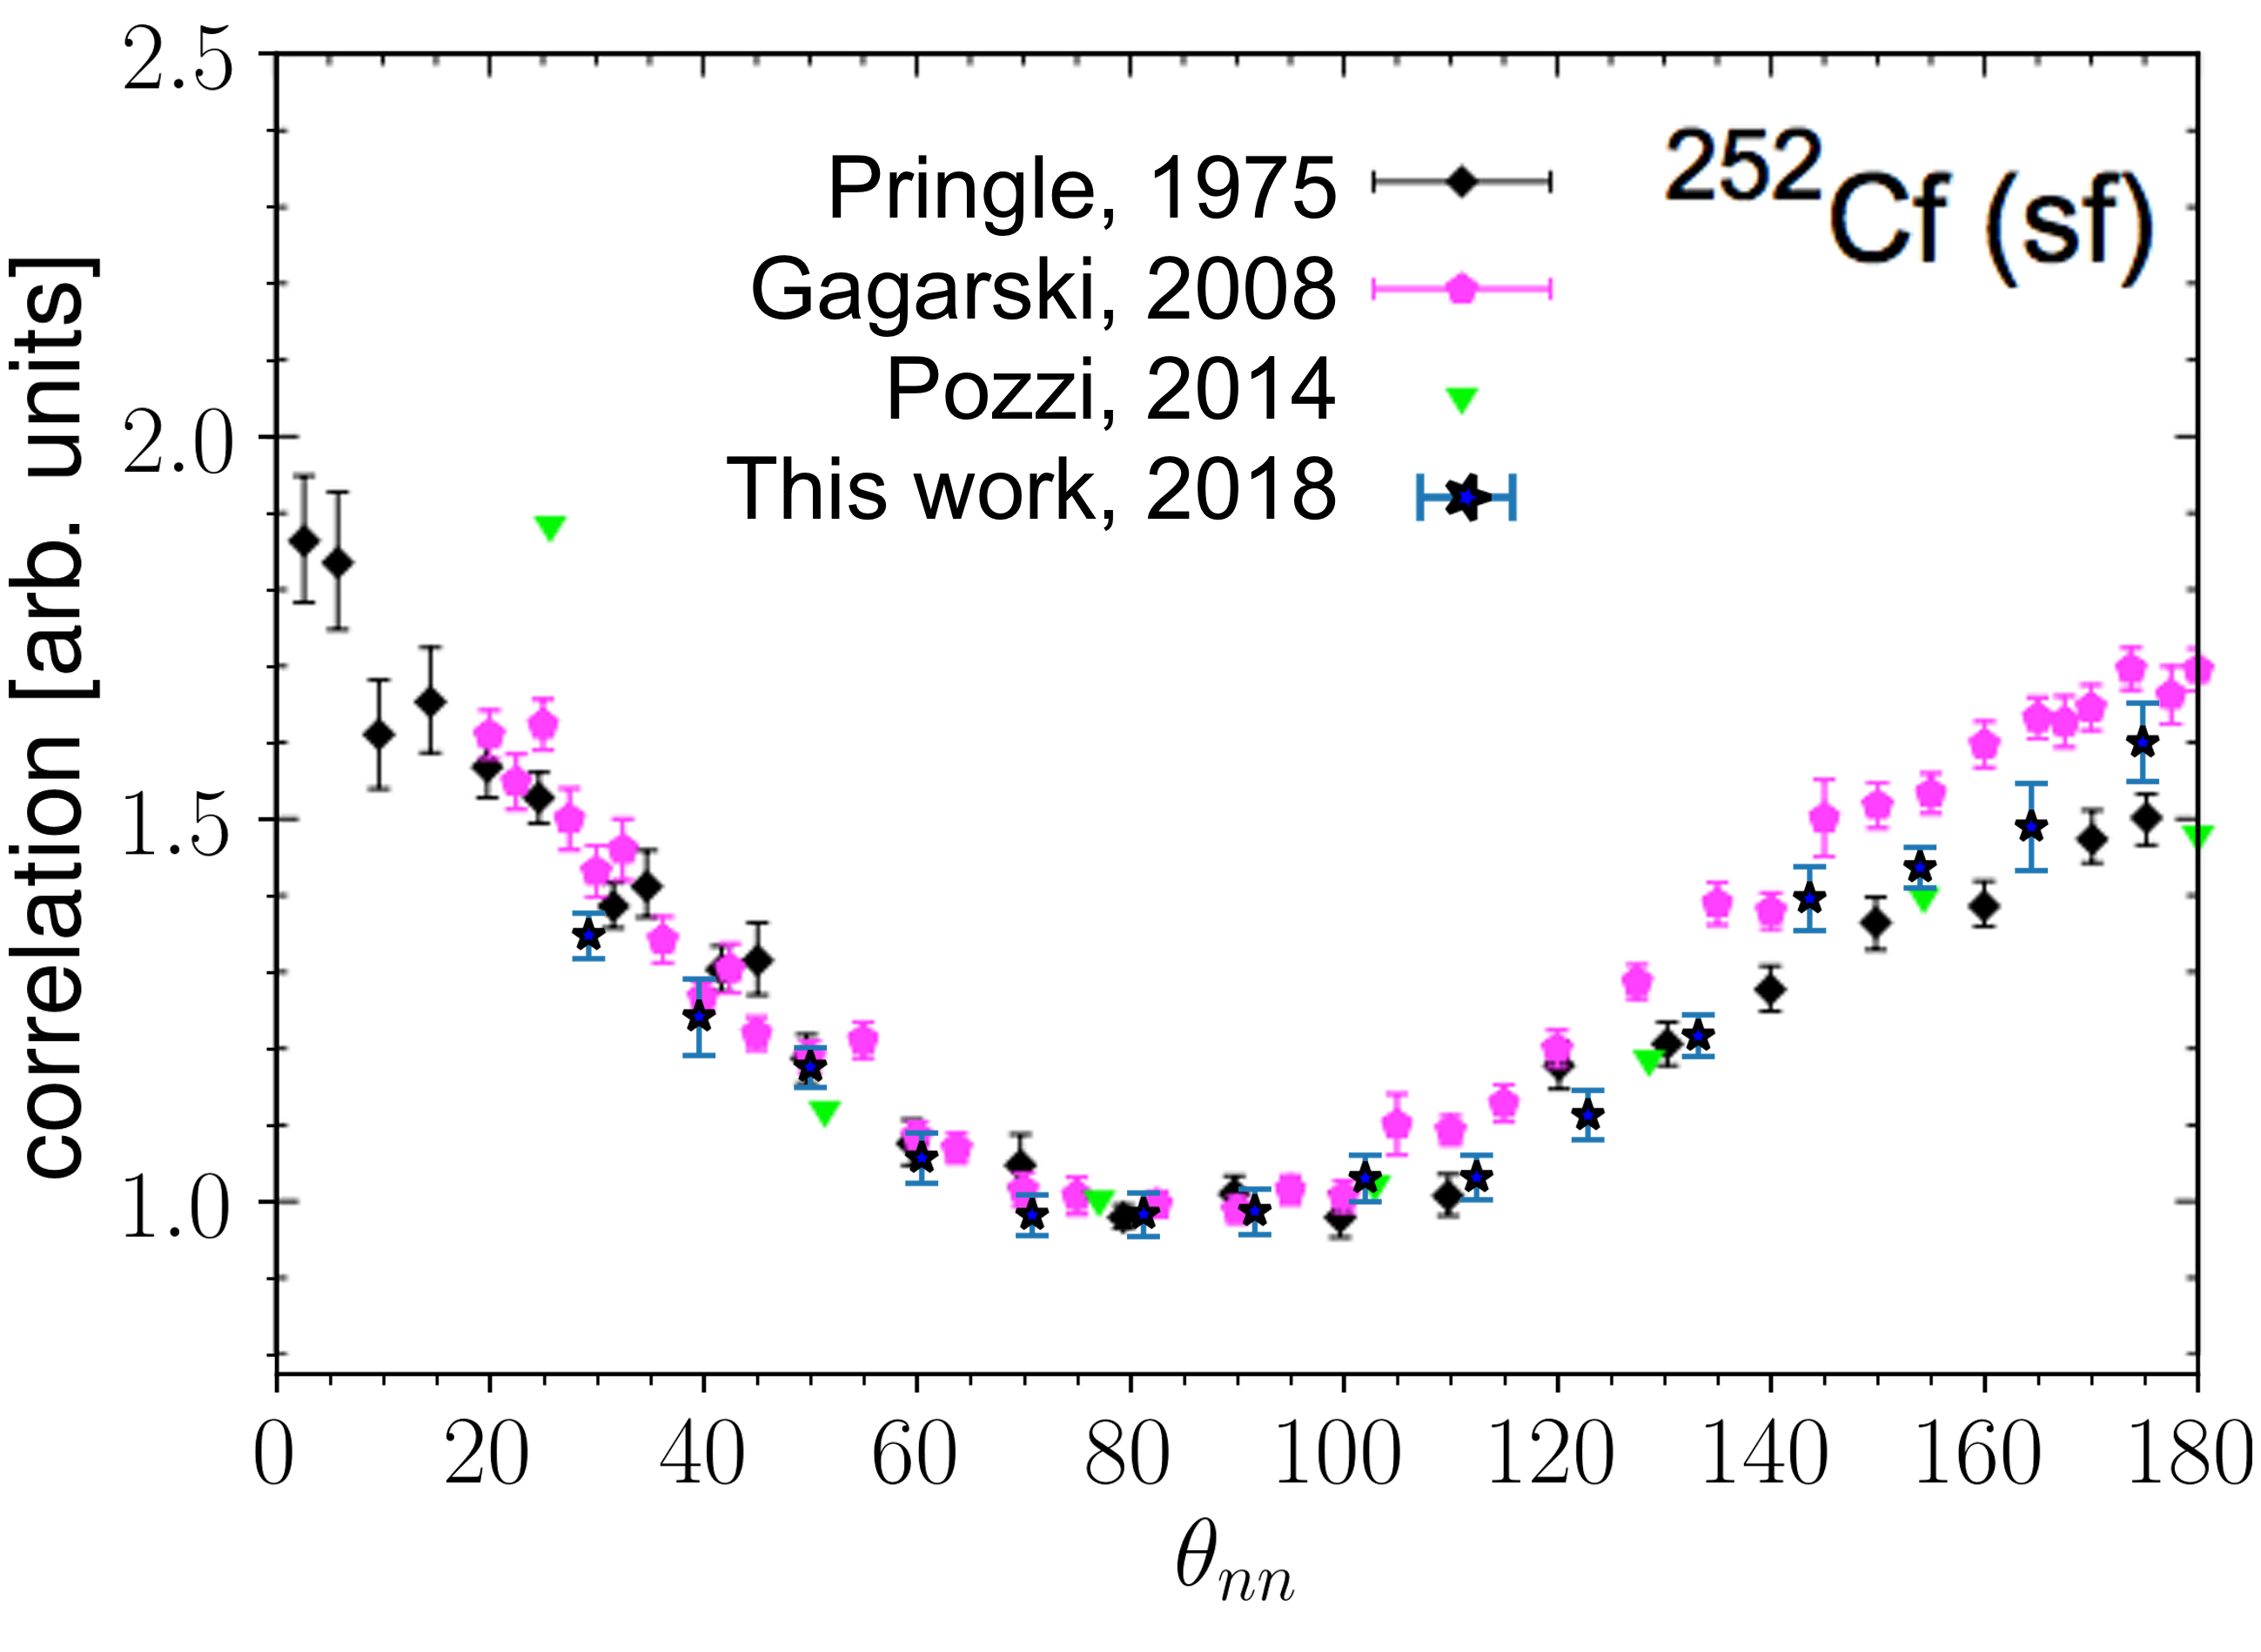
\includegraphics[width=0.7\textwidth]{Content/Introduction/Cf252_us_vs_them.png}
\caption{$\theta_{nn}$ distribution from the SF of $^{252}$Cf.
 The neutron detection threshold for Pringle~\cite{1975Cf252}, Gagarski~\cite{2008CF252}, and Pozzi~\cite{Pozzi2016} is 0.425 MeV, 0.425 MeV, and 0.7 MeV, respectively, and for this work is 0.5 MeV.
}
\label{fig:Cf252_us_vs_them}
\end{figure}

\chapter{Methods}


\section{Apparatus}
This experiment was carried out at the Idaho Accelerator Center (IAC), using their fast-pulsed linear accelerator, which is an L--band frequency (1300 MHz) electron linear accelerator.
It is capable of pulse widths ranging from 50 ps to 2 $\mu$s with a maximum energy of 44 MeV.
See section~\ref{beam} for the accelerator parameters used during the experiment.
Figure~\ref{fig:Facility} shows a top down diagram of the experimental arrangement.

\begin{figure}[h]
\centering
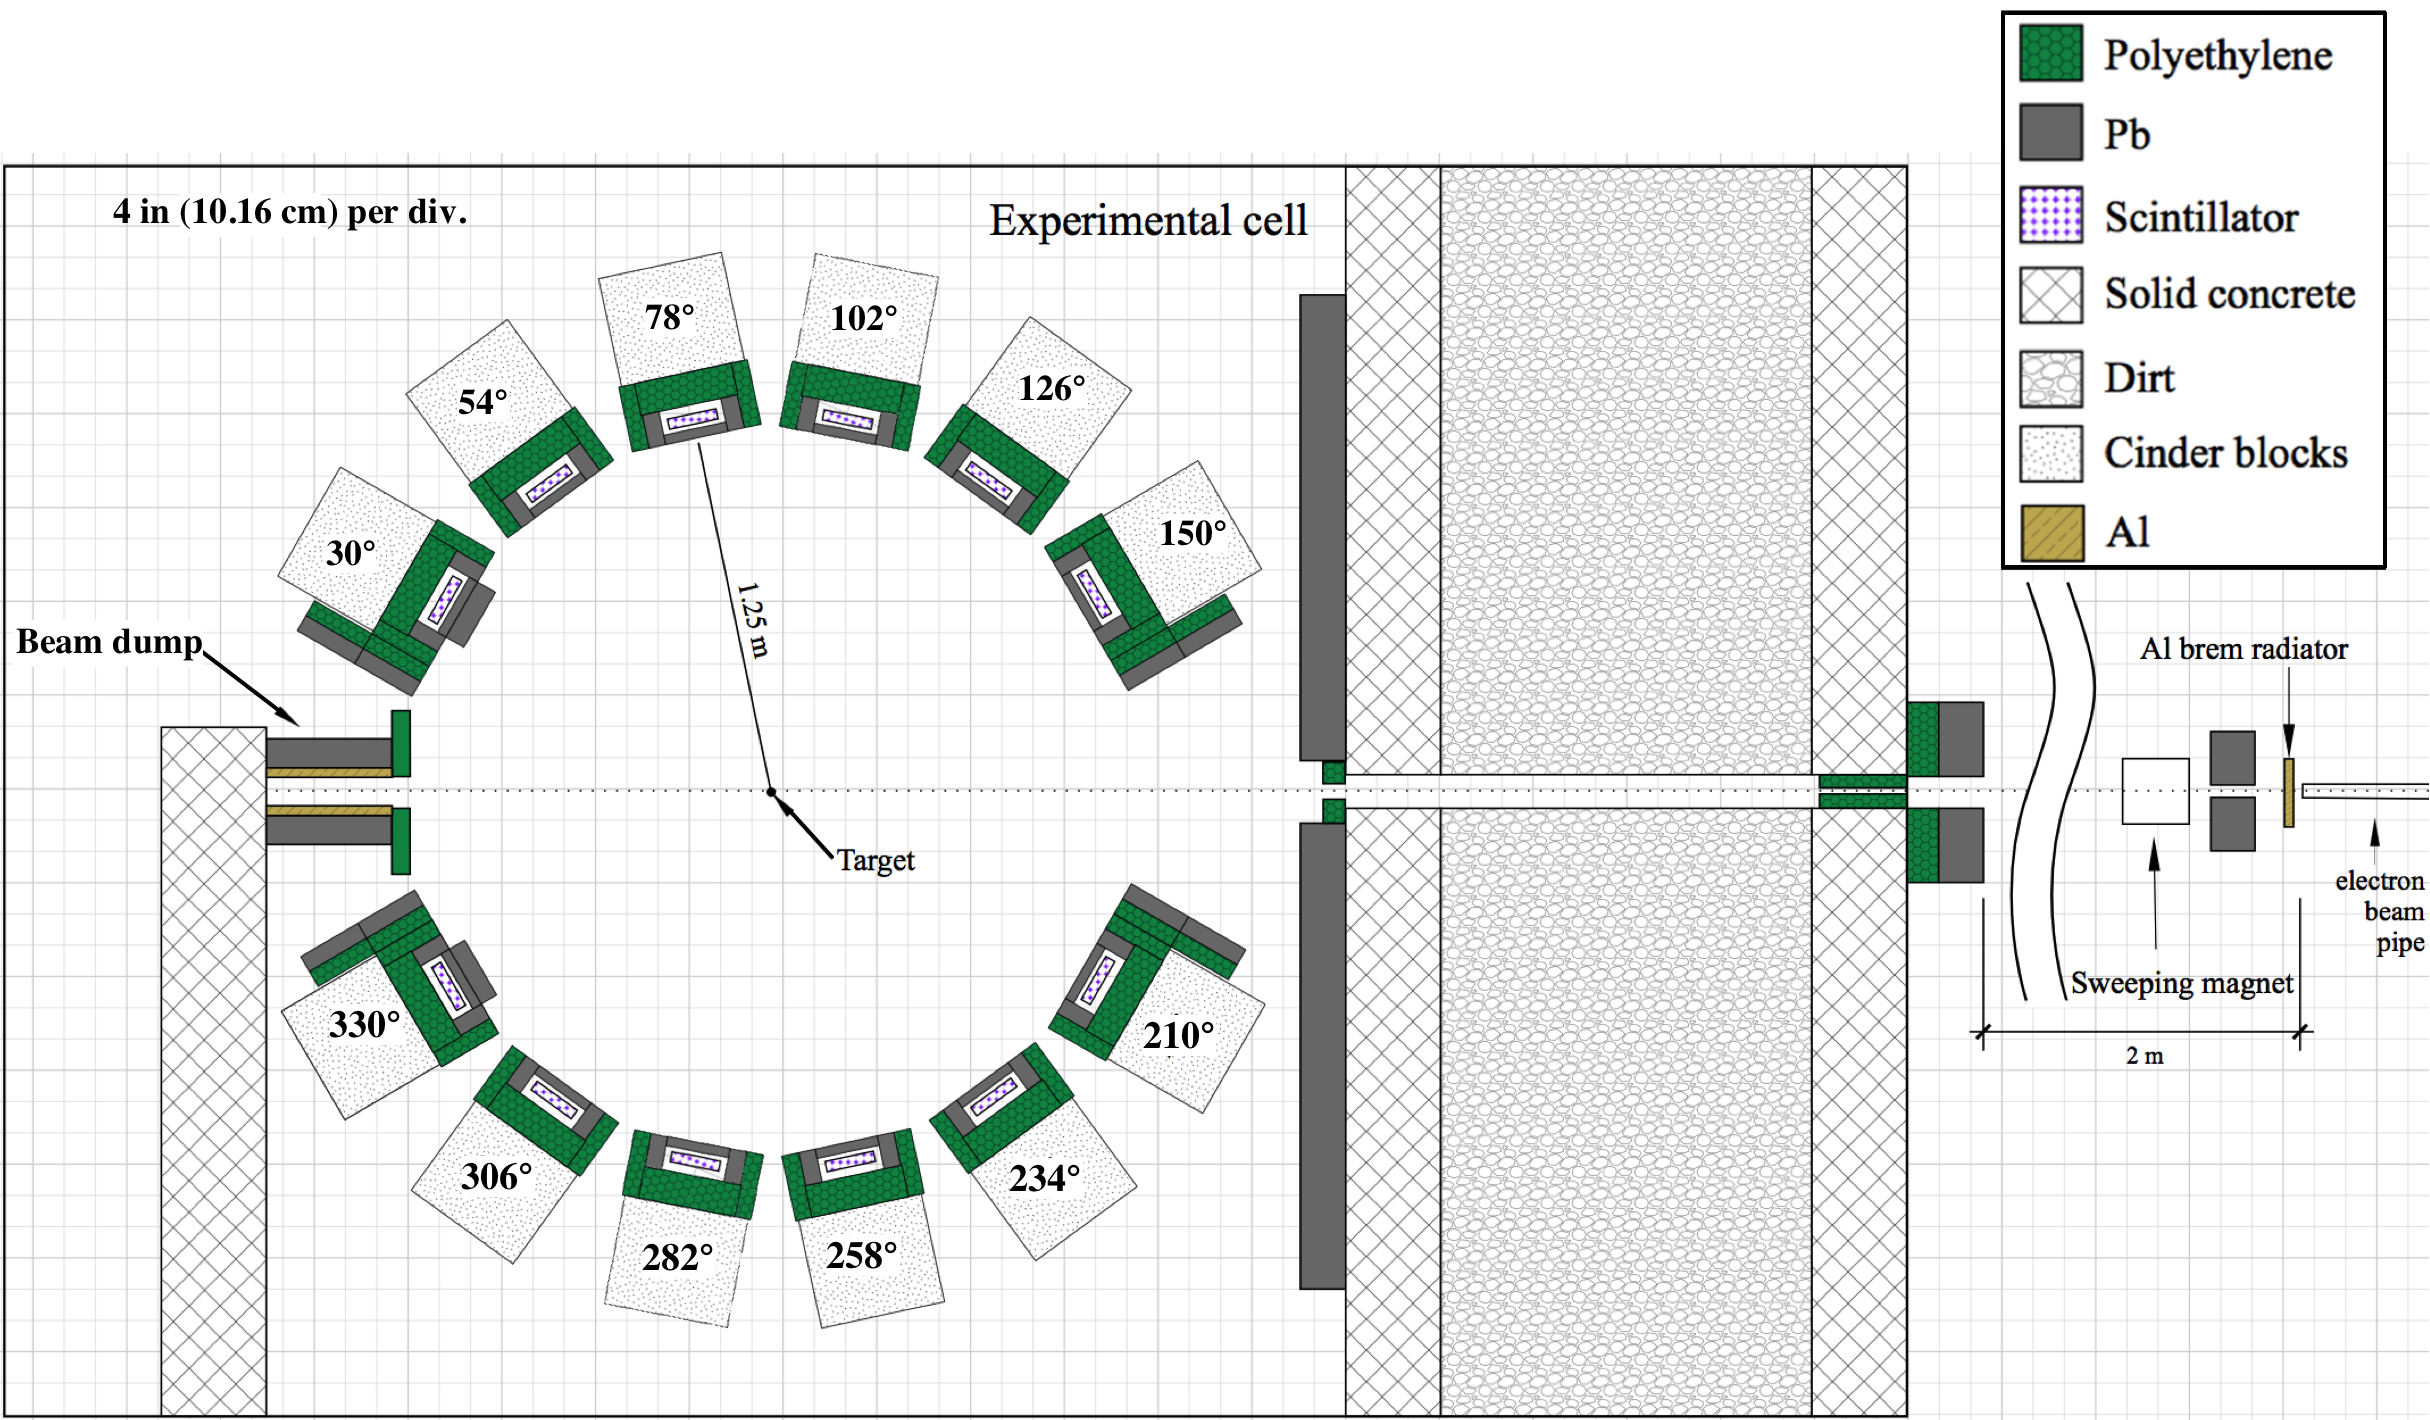
\includegraphics[width=0.95\textwidth]{Content/Methods/ExpArangment.jpg}
\caption{To-scale, top down diagram of the experimental setup.
An electron beam impinges upon a 3.8 cm thick Al radiator, and the resulting bremsstrahlung beam enters the experimental cell from the top.
The supporting structure for each detector has been labeled according to the angle, in degrees, between the center of each detector and direction of the incoming photon beam.
}
\label{fig:Facility}
\end{figure}
\subsection{Detectors}
\label{subsection:detectors}
The detection system measures neutron position and time of flight (ToF), which is defined as the time taken for a particle to travel from the target to any detector.
The purpose of the ToF measurement is to determine the kinetic energy of detected neutrons and to distinguish between photons and neutrons.
The detection system's positional precision is $\pm$9~cm, giving an average angular precision of $\pm6^{\circ}$ in the opening angles between the reconstructed positional coordinates of pairs of detected particles.

The neutron detection system consists of fourteen shielded scintillators arranged in a ring around the target (see Fig.~\ref{fig:DetGeom}).
The scintillators were made from Polyvinyl Toluene (PVT), an organic plastic scintillator.
Attached to both ends of each scintillator are 10-cm long, non-scintillating, ultra-violet transmitting plastic light guides.
A Hamamatsu 580-17 photomultiplier (PMT) tube is fixed to each light guide using optical glue.
In order to increase the chance that scintillation light remains inside the scintillator, they were polished to remove micro-imperfections and were wrapped in reflective aluminized mylar.

\begin{figure}[]
    \centering
    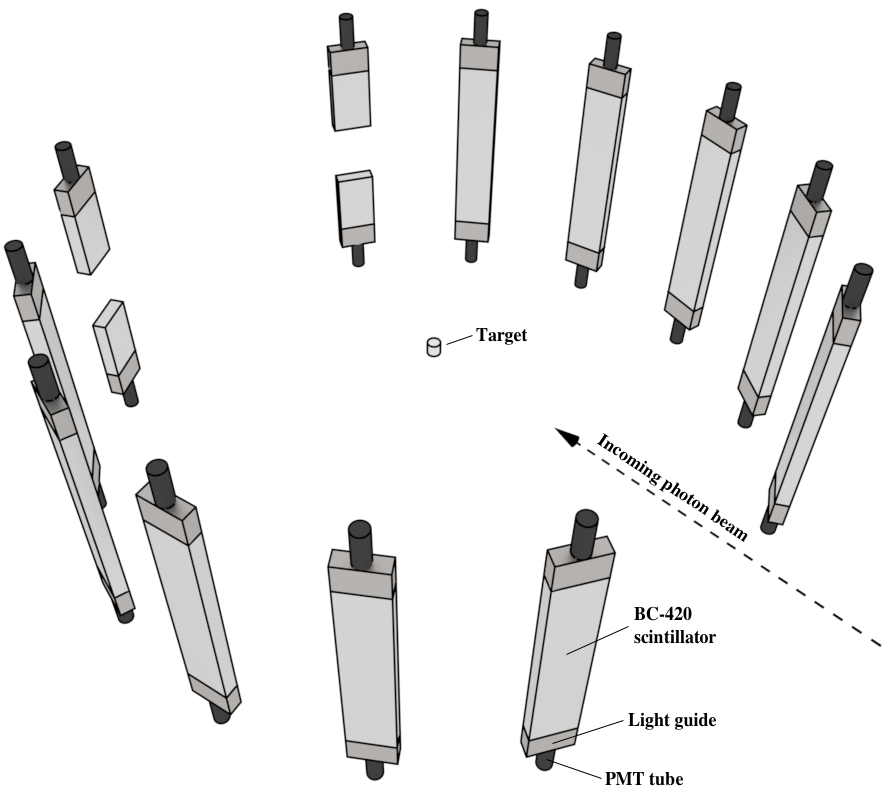
\includegraphics[width = 0.9\textwidth]{Content/Methods/Detectors.png}
    \caption{3-D render of the bare, unshielded scintillators, along with PMTs and light guides.}
    \label{fig:DetGeom}
\end{figure}

Ten out of the fourteen scintillators had dimensions of 76.2$\times$15.2$\times$3.8 cm$^3$.
The remaining four scintillators, with dimensions of 25.4$\times$15.2$\times$3.8 cm$^3$, were located at 30$^{\circ}$ and 330$^{\circ}$ with respect to the beam.
These scintillators were segmented in order to address very high photon detection rates resulting from the forward scattering of photons from the target.
Prior to segmentation, a photon was registered in these detectors nearly every pulse, and because the electronics were operated in single hit mode, the detection of a photon leaves the detector unable to detect subsequent neutrons, reducing the neutron detection efficiency to nearly 0\%.
After segmentation, the photon detection rate fell to 0.5 photons per pulse, greatly improving detector live-time.
The detectors at $\pm$30 degrees also differ from the rest in that they were instrumented with only a single PMT, and therefore have a lower energy and positional, and therefor angular, resolution than the others.
In order to test for systematic errors that may have resulted from the use of the segmented detectors, opening angle measurements were compared with and without their use, and the differences were well within experimental errors.

The relative efficiencies of the neutron detectors as a function of neutron energy were calculated by dividing measured and theoretical yields from the SF of $^{252}$Cf according to MCNP.
The results are shown in Fig.~\ref{fig:RelErgEfficiency}, which uses the aggregate of events from all detectors, and in Fig.~\ref{fig:RelErgEfficiencyVariation}, which shows it for each detector individually.
See section~\ref{Analysis} for a discussion of how the effects of detector efficiency are accounted for in this work.
\begin{figure}[]
    \centering
    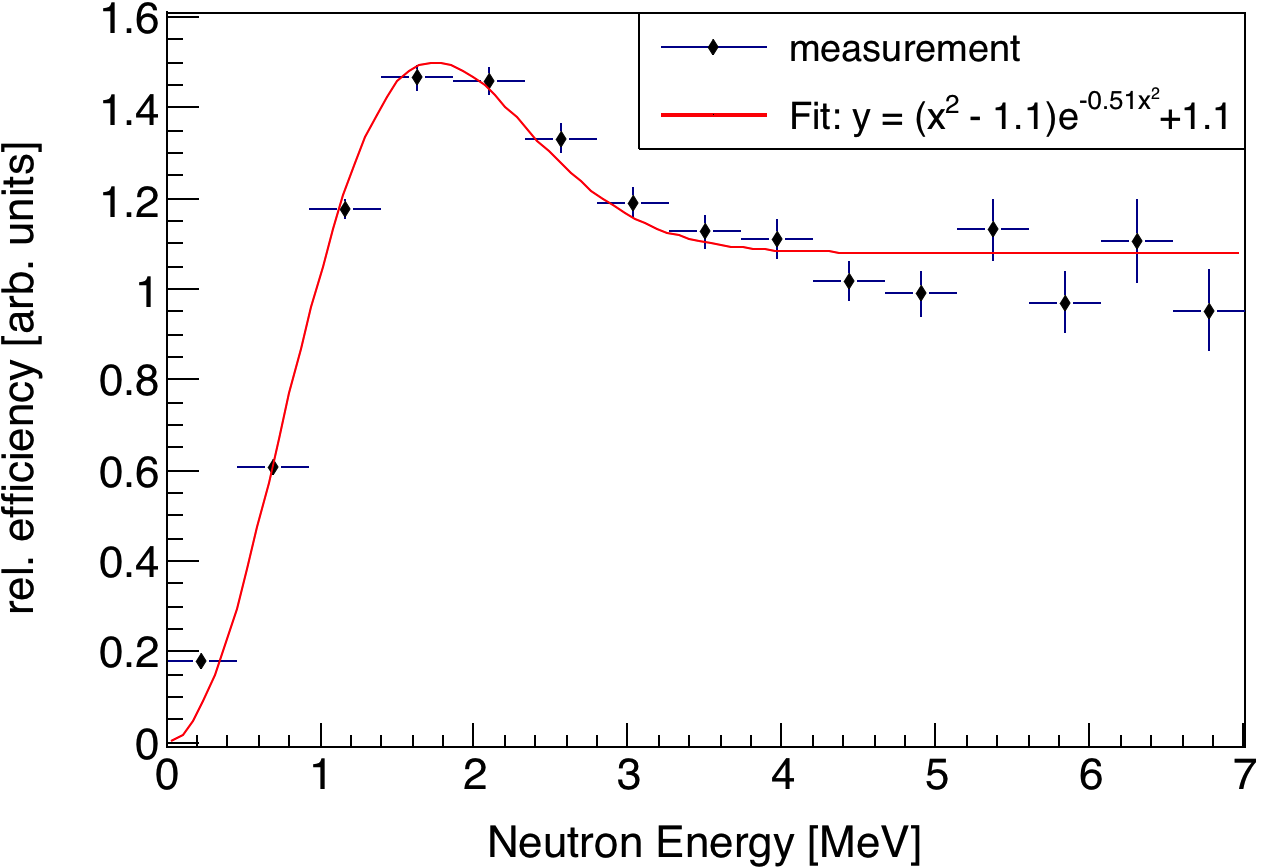
\includegraphics[width = 0.9\textwidth]{Content/Methods/RelErgEfficiency.png}
    \caption{The relative efficiency of the neutron detection system as a function of neutron energy is calculated by dividing the measured energy distribution by the theoretical energy distribution of neutrons from the SF of $^{252}$Cf.}
    \label{fig:RelErgEfficiency}
\end{figure}
\begin{figure}[]
    \centering
    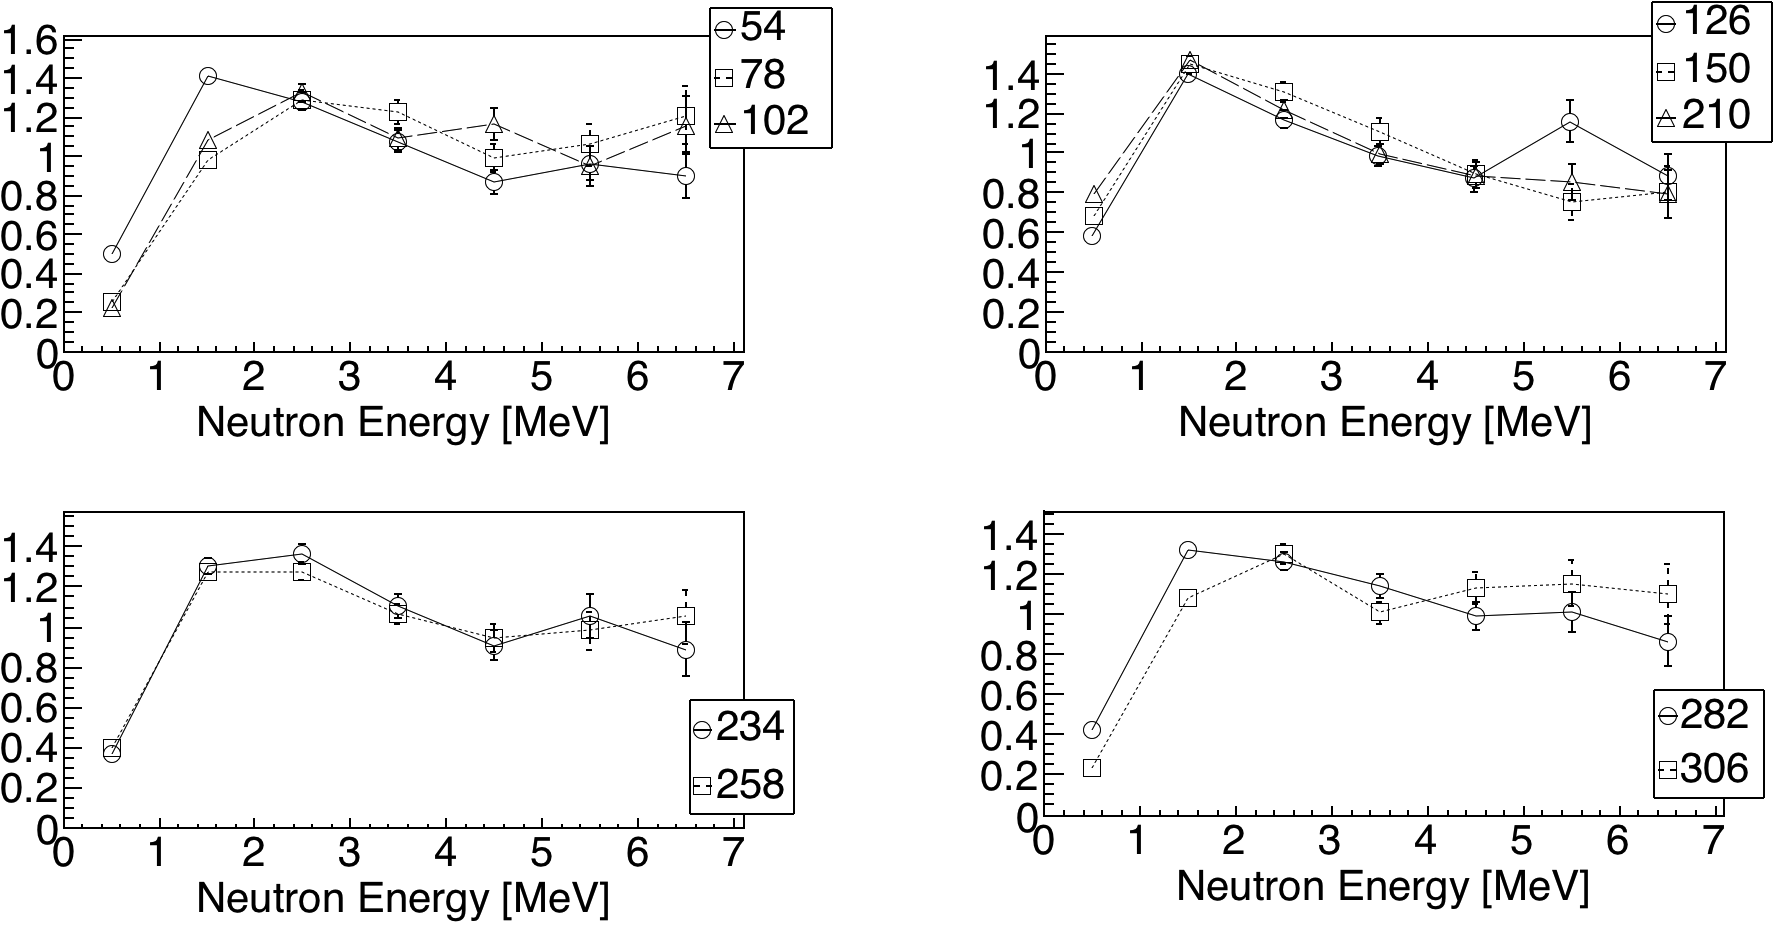
\includegraphics[width = 1\textwidth]{Content/Methods/RelErgEfficiencyVariation.png}
    \caption{
    The shape of the neutron detection efficiency curve varies among the detectors.
    The y-axis has arbitrary units and each curve is scaled to have the same integral.
    For the integrated neutron rates of each detector, see table~\ref{table:rates} in the appendix.
    Each detector is identified according to its angle relative to the photon beam, exactly as seen in Fig.~\ref{fig:Facility}.
    }
    \label{fig:RelErgEfficiencyVariation}
\end{figure}

\subsection{Detector Shielding}
\label{shielding}
\begin{figure}
    \centering
    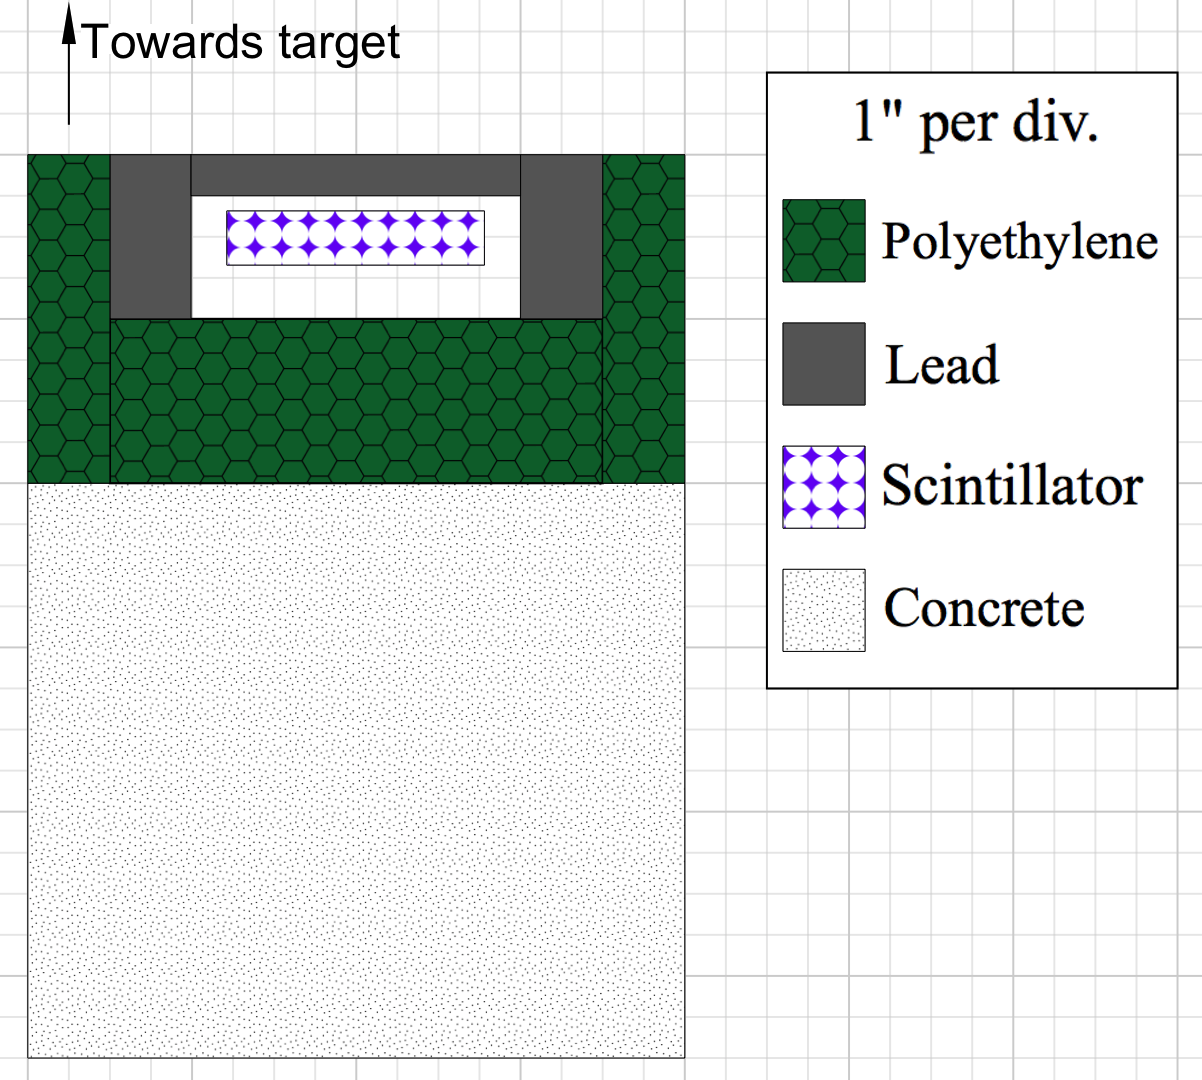
\includegraphics[width = 0.65\textwidth]{Content/Methods/DetShielding.png}
    \caption{Detector shielding was designed to reduce the detection of photons, room return, and detector cross-talk.}
    \label{fig:shielding}
\end{figure}
The detector shielding, depicted in Fig.~\ref{fig:shielding}, was constructed using lead and polyethylene with the aim of reducing cross-talk, the detection of photons, and noise.
Pb was used to attenuate photons, but has the side effects of neutron scattering and reduced neutron detection efficiency.
If a neutron scatters prior to being detected, the opening angle reconstruction and ToF calculation will be inaccurate because both assume that detected neutrons travel a straight path from the target to the detector.
2.5~cm of Pb was placed along the front face of the scintillators, which was enough to reduce photon detection rates to acceptable levels (see table~\ref{table:rates}), and, according to an MCNP simulation, leads to a root-mean-square error in opening angle and ToF of 1$^{\circ}$ and 0.3~ns, respectively, due to neutron elastic scattering.
The sides of each scintillator were shielded with 5 cm of Pb to attenuate photons, followed by 5 cm of polyethylene to reduce the chance of neutron cross-talk.
Also in order to minimize cross-talk, Pb was not placed behind the scintillators after an MCNP-POLIMI simulation indicated it would occur at significant rates otherwise.
Instead, 10~cm of polyethylene was placed behind the scintillators.
For a more detailed discussion about the issue of cross-talk, see section~\ref{crosstalk}.

\subsection{Bremsstrahlung Photon Beam}
\label{beam}
In order to ensure that all correlated neutrons produced are due to fission, the bremsstrahlung end-point was set to 10.5~MeV, safely below the ($\gamma, 2n$) threshold of 11.28~MeV for $^{238}$U.
Al was chosen for a bremsstrahlung radiator, because Al has a neutron knockout threshold above the energy of the electron beam, which ensured that the radiator would not be a source of fast neutrons with the potential to interfere with the experiment.
Downstream from the bremsstrahlung radiator is a sweeping magnet that removes charged particles from the photon beam.
Next, the beam traveled through a series of polyethylene and lead collimators and into the experimental cell in which the target was located (see Fig.~\ref{fig:Facility}).
Figure~\ref{fig:BremDist} shows the energy distribution of photons that reach the target according to an MCNP simulation that included the production and collimation of the bremsstrahlung photon beam.

The electron beam pulse width was set to 3~ns with a repetition rate of 240~Hz and a 1.1~A peak current.
The 3~ns pulse width was small compared to the median neutron ToF of 80~ns, and thus made a small contribution to the uncertainty in the neutron energy determination.

\begin{figure}[h]
\centering
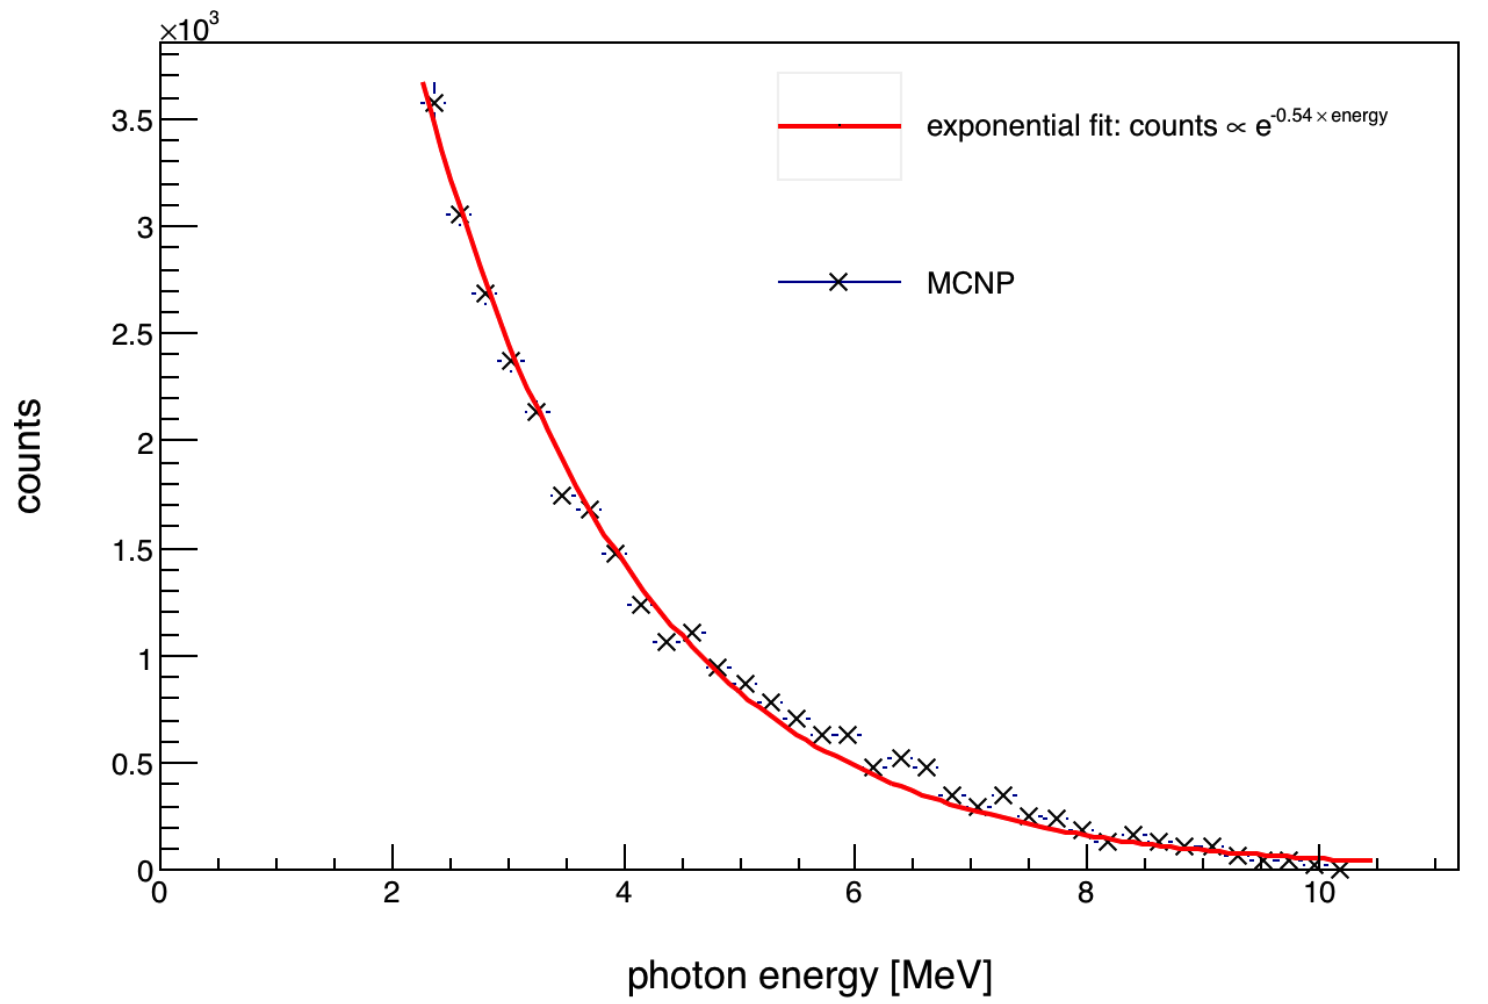
\includegraphics[width=0.7\textwidth]{Content/Methods/MCNPBremDistribution.png}
\caption{MCNP simulation of the energy distribution of photons that are incident on the fission target.}
\label{fig:BremDist}
\end{figure}

\subsection{DU Target}
\label{subsection:targets}
\begin{figure}[]
\centering
    \subfloat[]{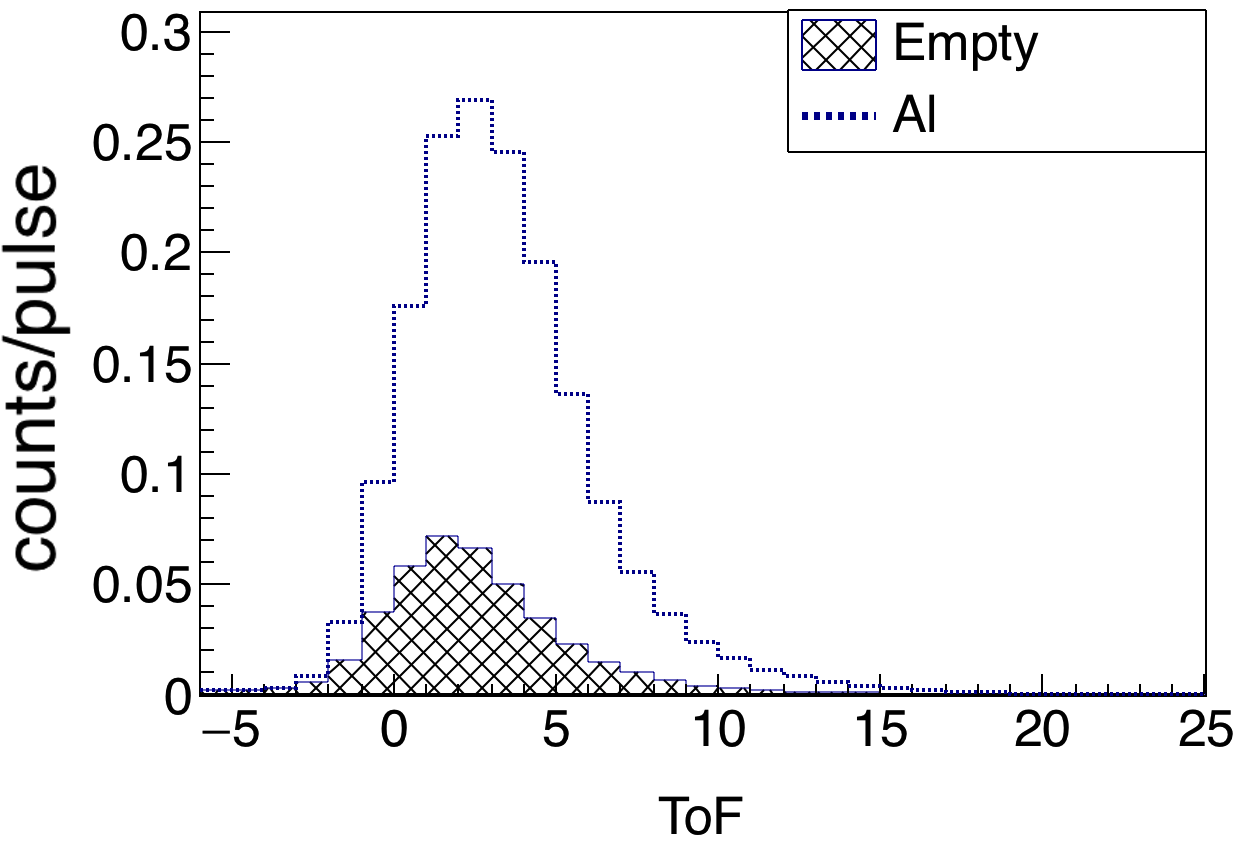
\includegraphics[width=0.5\textwidth]{Content/Methods/MTvsAl.png}}
    \subfloat[]{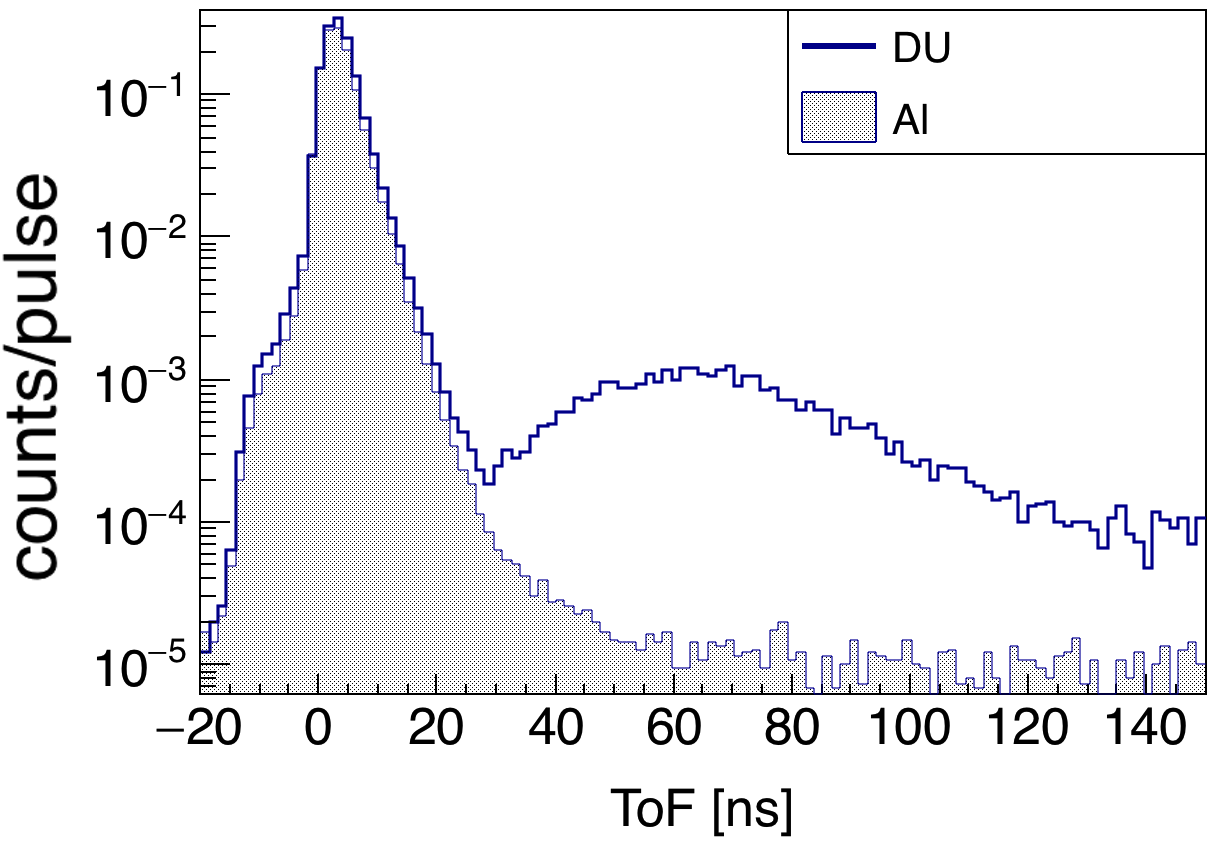
\includegraphics[width=0.5\textwidth]{Content/Methods/DUvsAl.png}}
    \caption{(a) Comparison between the ToF spectrum of a non-neutron producing target made from Al, to the ToF spectrum produced when no target is used.
    The large increase in events around 4~ns is due to photons that scatter from the Al target.
    When no target is in place, sources of the peak include the collimator leading into the experimental cell and the beam dump.
    The photon peak seen here is used to find the timing offsets that make it so $t=0$ corresponds to the moment of fission.
    (b) Comparison between the Al and DU targets show a pronounced increase in events between 35 and 130~ns due to the introduction of neutrons.}
    \label{fig:ToF}
\end{figure}
A depleted uranium (DU) target with dimensions of 4$\times$2$\times$0.05 $\text{cm}^3$ was used as the primary target.
DU received the majority of the allotted beam time because it is an even-even nucleus, and as a consequence, the fission fragments are emitted with a high degree of anisotropy~\cite{1977FragAss}.
Because the target lacked cylindrical symmetry, it was rotated slowly about the vertical axis during the experiment.
This was done in order to remove the potential for bias due to the elastic scattering of neutrons within the target.
See section~\ref{subsection:Elastic_scattering} for details.

\subsection{Electronics}
A data acquisition system based on NIM/VME standard was used.
A schematic of the data acquisition logic is shown in Figure~\ref{fig:WiringDiagram}.
The PMTs are supplied negative voltages ranging from 1300 to 1500 V by a LeCroy 1458 high voltage mainframe.
Analog signals from the PMTs were fed into a leading edge discriminator (CAEN Mod. N841) with input thresholds ranging from 30 mV to 50 mV.
The threshold and supply voltages were determined on a case by case basis for each detector so as to minimize noise, while also matching, as closely as possible, the efficiencies of all the detectors.
The logic signals from the discriminator were then converted to ECL logic and fed into a CAEN model V1290A TDC.
The timing of signals from the PMTs were always measured relative to a signal from the accelerator provided at the beginning of each pulse.
Even though a multi-hit TDC was being used, only the first signal from any given PMT is used each pulse due to concerns over signal reflections within the cables.
On the software side, the CODA~\cite{CODA} software package developed by Jefferson Laboratory was used to read out the data from the TDC and digitally store it for analysis.

\begin{figure}[h]
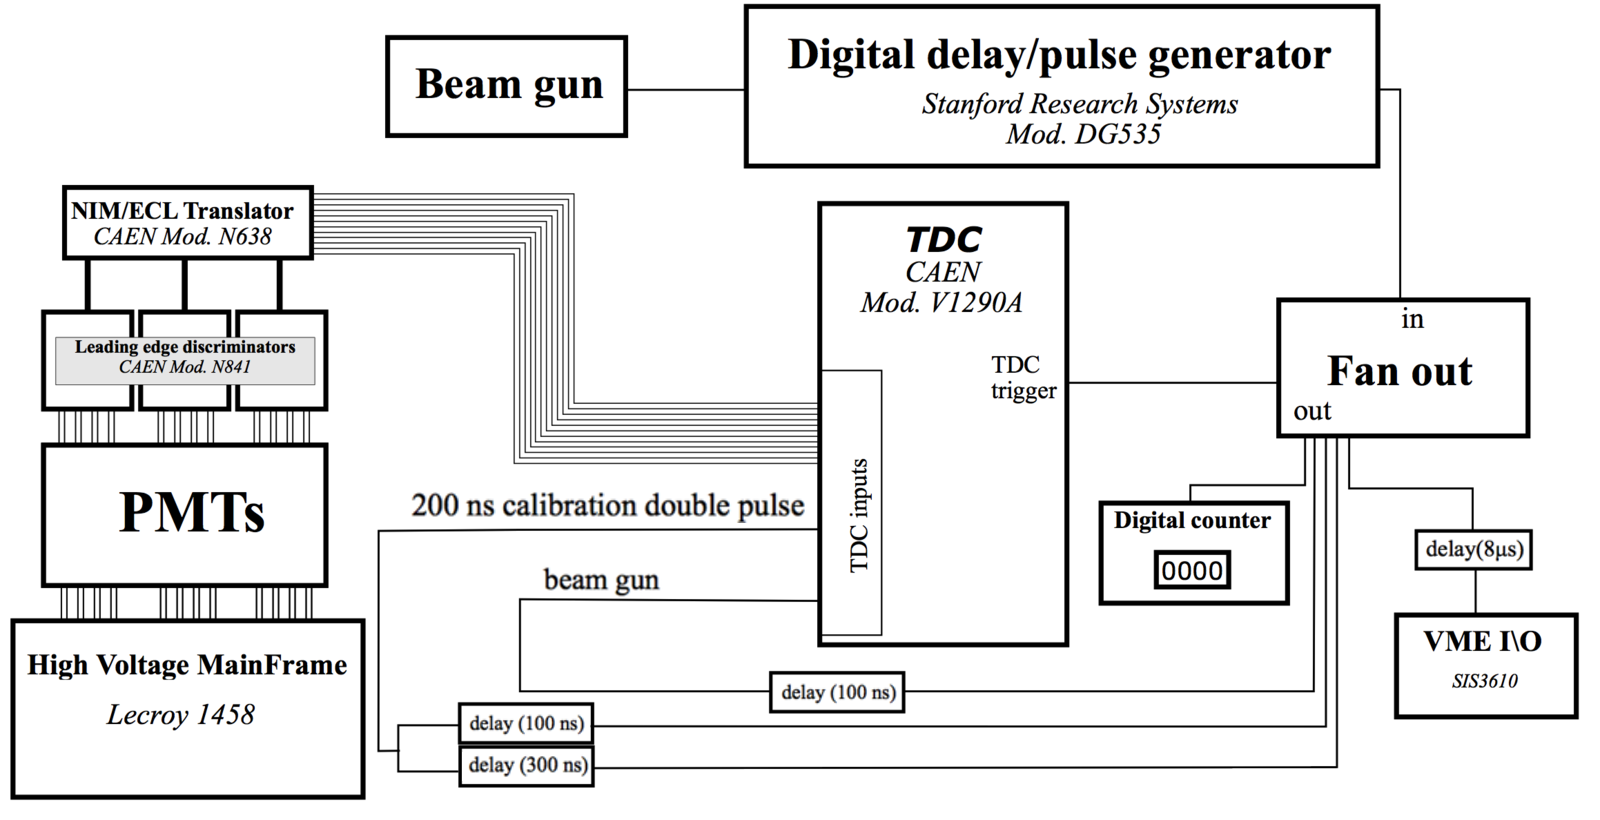
\includegraphics[width=0.9\textwidth]{Content/Methods/WiringDiagram.png}
\caption{Wiring diagram of the electronics setup. }
\label{fig:WiringDiagram}
\end{figure}

\section{Experimental Methods}
\subsection{Photon Beam}
The accelerator's pulse width is set to 3 ns, where as the fastest and slowest neutrons in this experiment have a time of flight of 40 ns and 130 ns, respectively.
A bremsstrahlung photon beam is produced by the passage of 10.5 MeV electrons through a 1" thick slab of aluminum.
Aluminum was chosen as the radiator because it has a neutron knockout threshold above the energy of the 10.5 MeV electron beam.
This prevents the bremsstrahlung radiator from being a source of fast neutrons, which could have the potential to travel into the experimental cell and cause false neutron events.
Downstream from the bremsstrahlung radiator, a sweeping magnet removes excess electrons from the photon beam (see figure~\ref{fig:Facility}).
Before reaching the experimental cell, photons are collimated by a series of polyethylene and lead collimators aimed at eliminating beam contaminants.

** ToDo: Think about if/where to include the calculation of the ratio of knockout neutrons to fission neutrons.
Have only done calculation for Thorium.

When attempting a measurement of prompt neutrons from photofission, an ambiguity can arise between neutrons from photofission and neutrons from $(\gamma, xn)$.
This is because the two reactions have similar cross-sections within the GDR region.
Furthermore, there is significant overlap between the energy spectra of the neutrons from $(\gamma, xn)$ and photofission.
Since this measurement is concerned only with observing two neutrons in coincidence, it suffices to set the Bremsstrahlung end-point at 10.5 MeV, since this value is below the threshold for ($\gamma, 2n$) of our targets ($\sim$12 MeV).
Using an and-point of 10.5 MeV still leaves the possibility of the detection of multiple ($\gamma, 1n$) reactions in a single pulse, but this is an accidental coincidence.
An \textit{accidental} neutron coincidence occurs when two uncorrelated neutrons happen to be detected in the same pulse.
All accidentals follow Poissonian distribution, allowing for their subtraction from the data.
The details of the procedure used to subtract accidentals is explained in section~\ref{Subtraction of Accidentals}.

The energy distribution of photons reaching the target was simulated using MCNP.
The creation and collimation of the Bremsstrahlung photons in included in the simulation.
The resulting energy distribution is shown in figure~\ref{fig:BremDist}.

\begin{figure}[h]
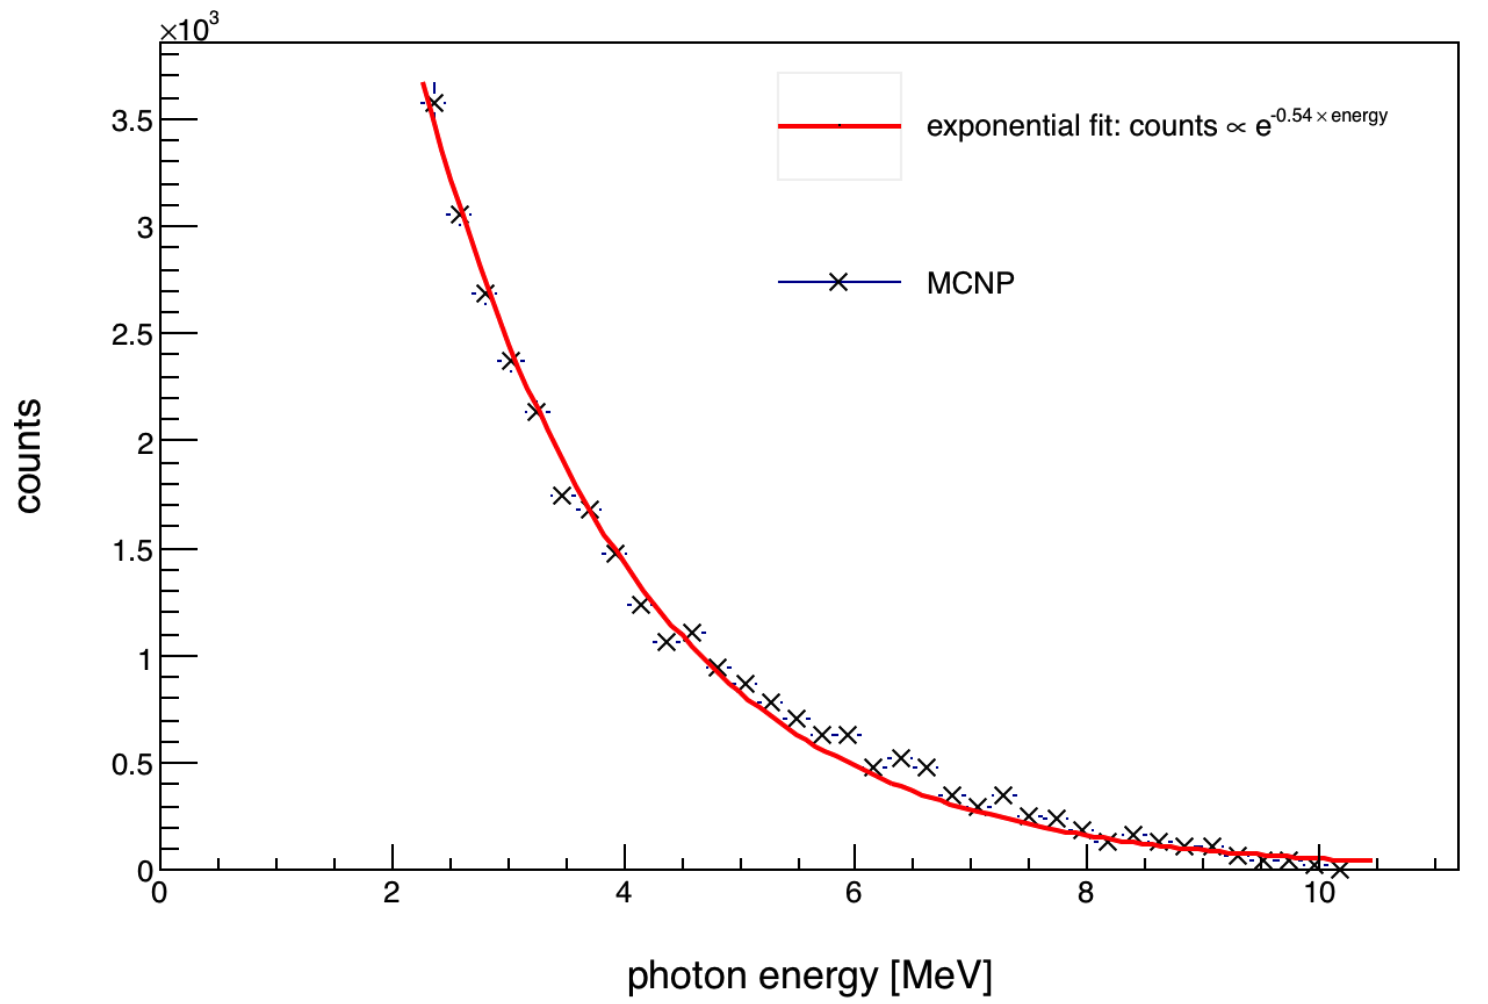
\includegraphics[width=0.9\textwidth]{Content/Methods/MCNPBremDistribution.png}
\caption{Result of an MCNP simulation of the energy distribution of the Bremsstrahlung photons that reach the target. Points are from the simulation, and the line is an exponential fit ($Ae^{-bx}$). The constant of proportionality, $A$, is arbitrary. The value for $b$ is 0.54.}
\label{fig:BremDist}
\end{figure}

The electron pulse width was set to 3 ns and had a 1.1A peak current, with a repetition rate of 240 Hz.
The 3 ns pulse width was not a significant source of error in the measurements of neutron time of flight, since neutron events had a median time of flight of about 80 ns.
The accelerator current is set by requiring there be, on average, fewer than one fission per pulse, thereby reducing the detection of uncorrelated neutrons from multiple fissions occurring in a single pulse.
Even so, the detection of uncorrelated neutrons is unavoidable because of statistical fluctuations.
To address this, a technique is developed to subtract these events from the data (see section~\ref{Subtraction of Accidentals}).

**ToDo Discussion about the LINAC's low duty factor??

\subsection{Particle time of flight determination}
\label{reconstruction}

%python file: ProductionAnalysis/TOFGraphs
\begin{figure}[htbp]
\begin{center}

\subfloat[$\Delta T$s with no target in place. ]{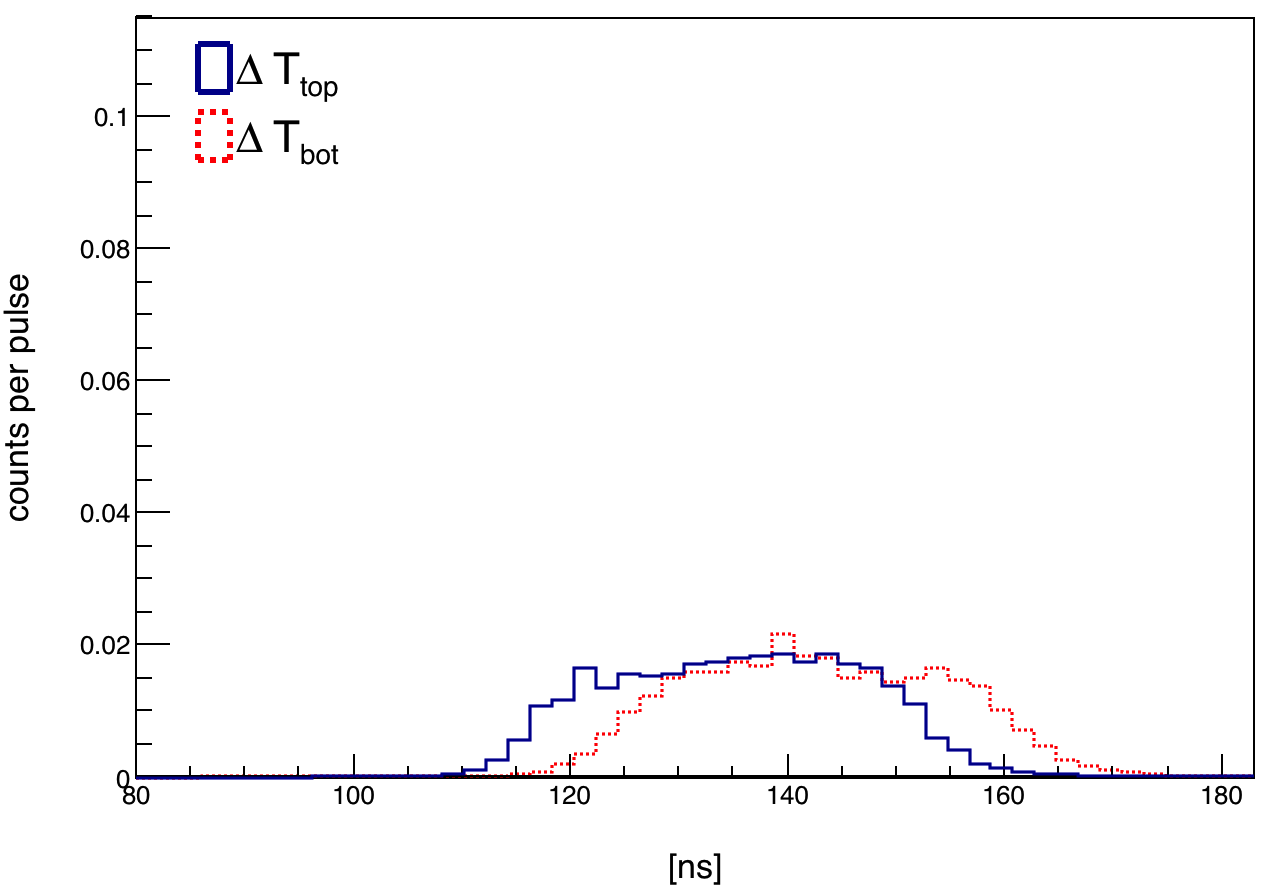
\includegraphics[width=0.5\textwidth]{Content/Methods/ToF0.png}}
\end{center}

\subfloat[$\Delta T$s with Aluminum target.]{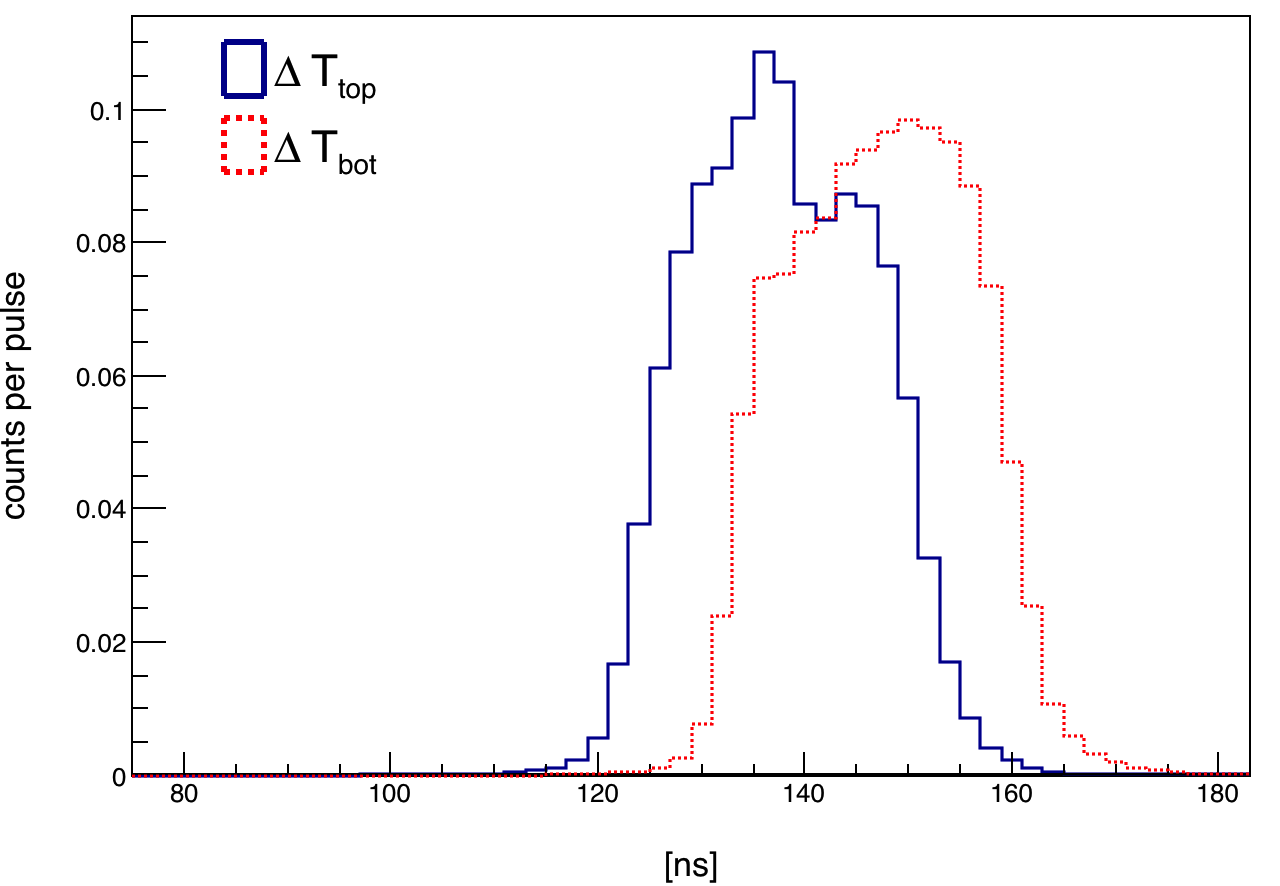
\includegraphics[width=0.5\textwidth]{Content/Methods/ToF1.png}}
\subfloat[Average of $\Delta T_{\text{top}}$ and $\Delta t_{\text{bot}}$  with Aluminum target in place.]{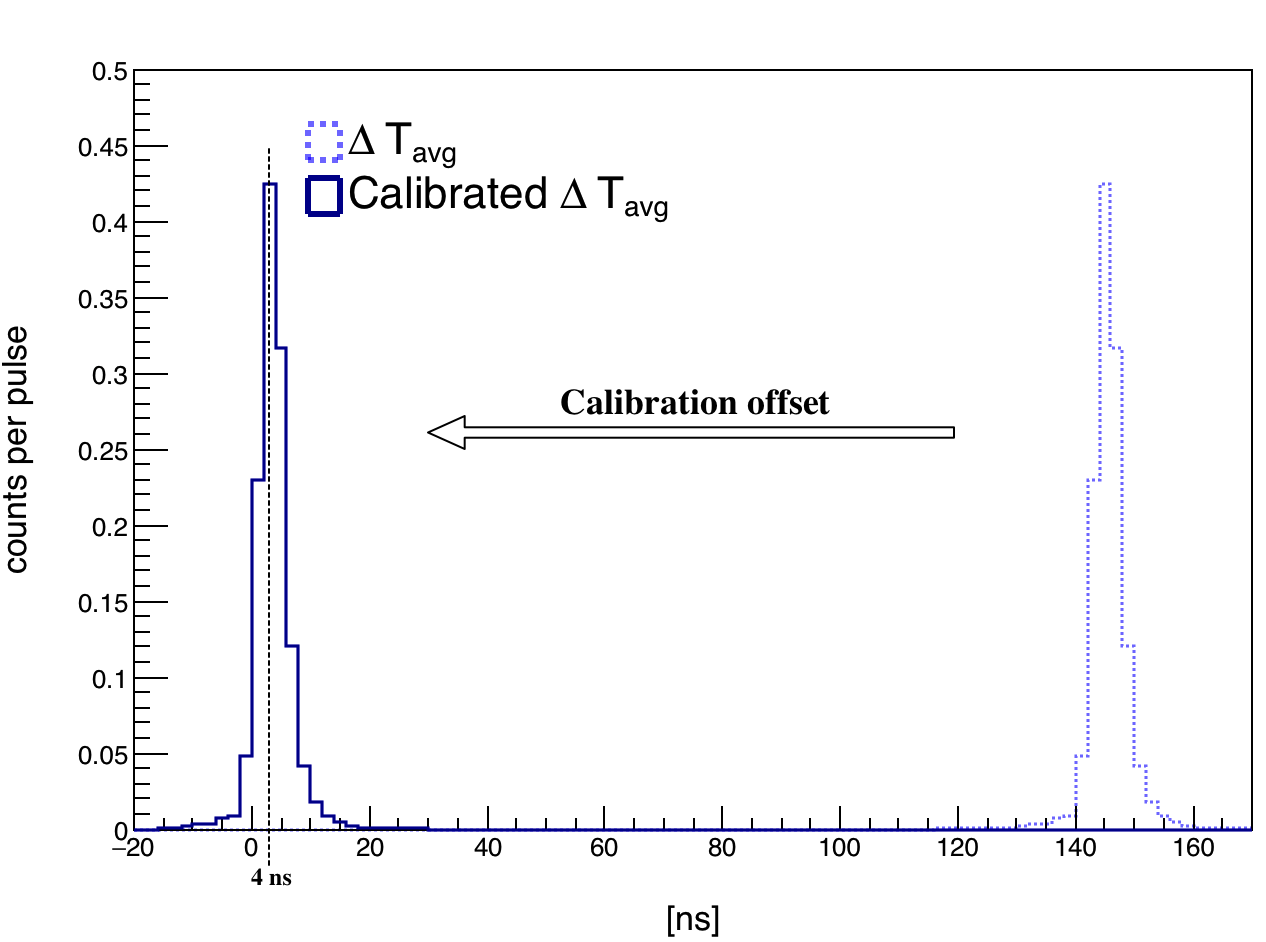
\includegraphics[width = 0.5\textwidth]{Content/Methods/ToF2.png}}
\caption{(a) The $\Delta T $ spectra of PMTs with no target in place  shows the background produced by the beam alone.
(b) Using Aluminum as a non-neutron producing target, a peak appears in each spectra caused by photons scattering from the target.
Since these photons travel a known distance of 1.25 m between the target and detector face, the width of these spectra reflect the range in scintillation light propagation times along the 76.2 cm length of the detector.
(c) Taking the average of the $\Delta T$s of the top and bottom PMTs produces a sharp peak, since the sum of the scintillation light propagation times from both PMTs is always equal to the time required for light to travel the detector's full length.
The correct timing offset can be then be found using using the fact that photons have a time of flight of 4 ns. }
\label{fig:ToFDetermination}
\end{figure}

Each detector was equipped with two PMTs fixed on opposite ends of the scintillation cell, with the exception of the detectors located farthest downstream at $\pm30^{\circ}$, which only had a single PMT.
The PMTs provide a signal in response to scintillation light with timing resolution of less than 1 ns.
However, the main source of uncertainly in the time of a particle hit is variation in the time taken for scintillation light to propagate to the PMTs. No pulse shape discrimination was used in this study.
Particle identification, along with the reconstruction of energy and position was achieved solely from the timing of signals from PMTs.
The time of each event in a PMT was measured relative to a signal provided by the accelerator at the beginning of each pulse, which is referred to as the \textit{beam gun}.

Time of flight (ToF), the time for a particle to travel from the target to the face of a detector, was used to distinguish between photons and neutrons, and to measure neutron energy.
The time of flight was calculated by taking the average between the times of signals from the top and bottom PMTs, and subtracting an offset determined from a calibration.
In the detectors located at $\pm30^{\circ}$, which have only one PMT, ToF is calculated from the timing of events in its sole PMT, minus a calibration offset.

The ToF of a particle that causes coincident events in both PMTs of a detector, obeys the following relationship:
\begin{displaymath}
ToF = C_i + \Delta t_{\text{avg}} 
\end{displaymath}
where $\Delta t_{\text{avg}} $ is the average between the timing from the top and bottom PMTs, and $C_i$ is a constant timing offset that is the same for every pulse.
The subscript on $C_i$ is used because the timing offset is different for each detector.
Any process that produces a timing delay that does not change from pulse to pulse contributes to $C_{i}$.
Examples of this are the time required for photons to travel from the bremsstrahlung radiator to the target, the propagation of signals through the wires connecting the PMTs, and delays in the electronics for processing.

The time required for scintillation light to travel through the detector, from point of scintillation to a PMT mounted at the detector's top or bottom, can vary from 1 ns for particles that hit very close to a given PMT, to about 8 ns for particles that hit across the detector from a given PMT. The sum of the times taken for scintillation light to travel to the top and bottom PMTs is just the time taken for the light to travel the full length of the detector, which is nearly constant.
The rate at which light propagates along the length of a detector is dependant on speed of light in the material and the light's flight path.
The flight paths of detected scintillation light tend to be parallel to the long axis of the detector, because these paths are the shortest possible, and only the first signal from a PMT is accepted.
Therefore, by taking the average of the times in the top and bottom PMT, the time required for scintillation light to propagate through the scintillator becomes a constant offset.

The validity of a constant scintillation light propagation time was verified experimentally using a $^{60}Co$ source.
With the face of the scintillator covered with 2" thick bricks of lead shielding, the $^{60}Co$ source is placed against the lead at several locations along the length of the detector.
The lead brick between the $^{60}Co$ source and the scintillator has a small hole drilled through it, giving the $^{60}Co$ a direct line of sight to a point on the face of the scintillator.

**ToDo: Make a figure for the setup of the co60 calibration. 

\begin{figure}
    \centering
    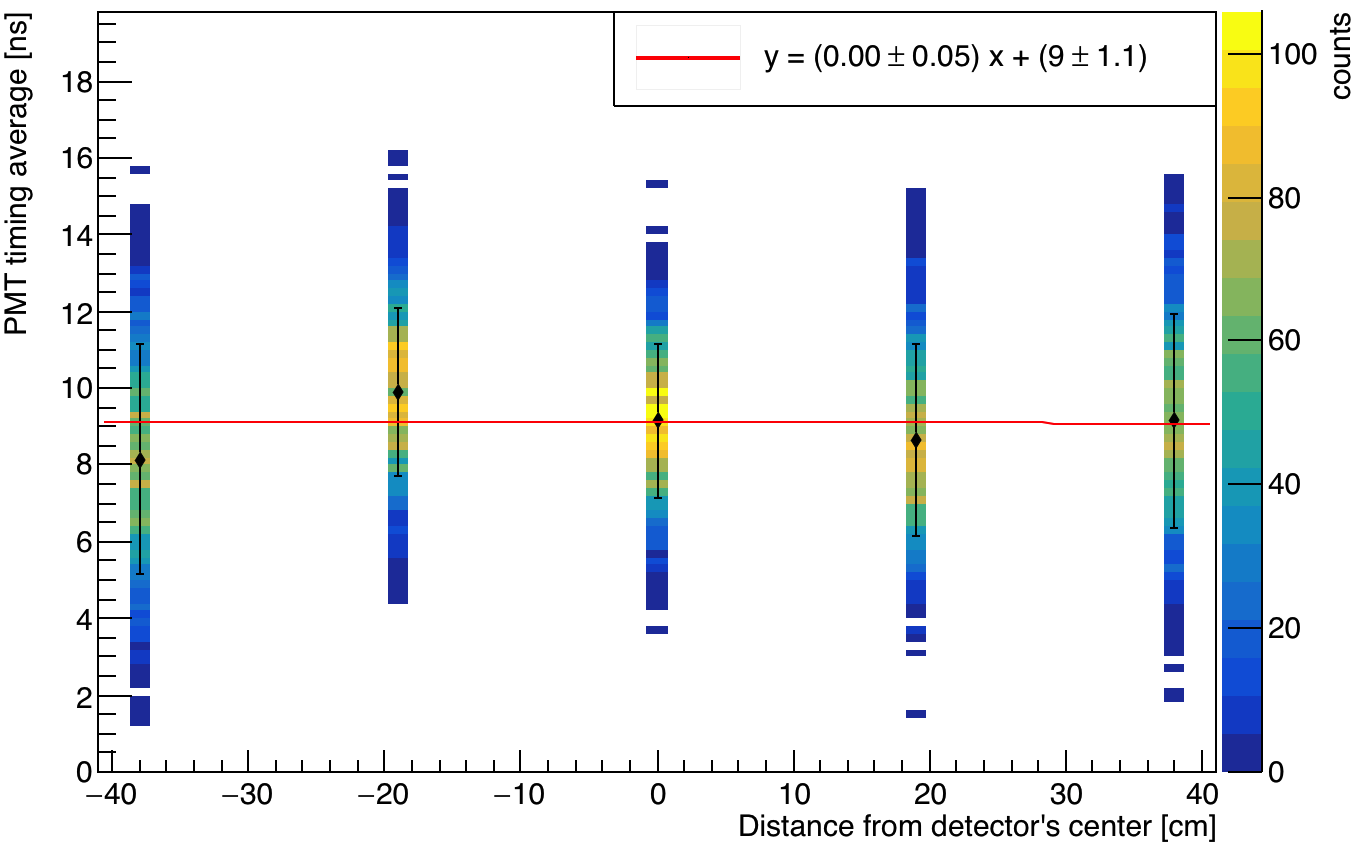
\includegraphics[width = 0.9\textwidth]{Content/Methods/CO60Validation.png}
    \caption{A $^{60}Co$ source, which emits coincident back-to-back photons, is placed at several positions along the face of a lead shielded scintillator.
    At each position, a small hole is drilled through the lead to give the $^{60}Co$ source a line-of-sight to a well-defined point on the scintillator.
    Then, a high timing resolution photon detector is placed close to the $^{60}Co$ source.
    $^{60}Co$ decays to emit two photons simultaneously--one photon is detected by the high timing resolution detector and serves as the ``start'' time, and the other photon causes a scintillation event in the detector being calibrated .}
    \label{fig:Co60Validation}
\end{figure}

\begin{figure}
    \centering
    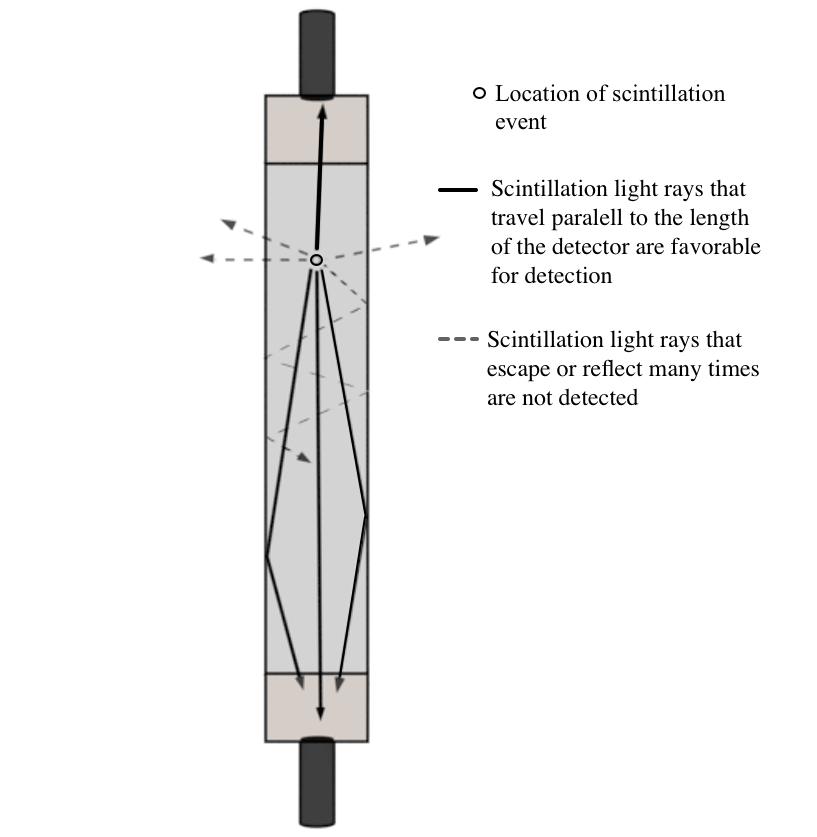
\includegraphics[width = 0.8\textwidth]{Content/Methods/lightpaths.png}
    
    \caption{Hypothetical paths of light rays as they propagate through the scintillator after a scintillation event.
    The light rays that first reach a PMT (solid) travel a shorter path than the others (dotted), and thus experience the least amount of attenuation.
    This experiment always uses the first signal from a PMT and hence the data favors cases in which scintillation light travels a short path to a PMT.
    In other words, the detectors favor the detection of scintillation light that is traveling parallel to the long axis of the detector.
    As a result, the sum of the times required for scintillation light to reach both PMTs is just the time taken for light to travel the full length of the detector, which is a constant.
    Thus, by taking the average time between coincident events in both PMTs, the time required for the propagation of scintillation light becomes a constant that is removed during calibration.
    ** ToDo: Consider removing this figure  }
    \label{fig:lightpath}
\end{figure}

The value of the constant offset for the calculation of ToF is determined by observing photons that are known to have scattered from the target. Comparing the timing spectra of a non neutron producing target made from aluminum, to the spectra produced when no target is used reveals a prominent peak caused by the photons that scatter from the target. The distance these photons must travel to reach the center of a face of any detector is 125 cm, and 130 cm to reach the top or bottom edges of a detector. It takes light 4.1 ns and 4.3 ns to travel 125 cm and 130 cm, respectively. The difference between these two ToFs is negligible compared to experimental uncertainty, so the ToF of photons that scatter from the target is assumed to be 4 ns, and with this assumption the constant timing offset of each detector can be calculated.  
   
\subsection{Particle position reconstruction}
Spacial resolution in the horizontal plane is determined by the physical dimensions of the detector. It's dimensions in the horizontal plane are comparatively small being 3.8x15 cm$^2$, so it suffices to use the geometric center of the detector as the horizontal component of a detected particle's position. In doing this, a positional uncertainty of $\pm$7.5 cm is introduced, which in terms of an opening angle is $\pm4^{\circ}$. The final results of this work use an opening angle bin width of 20$^{\circ}$, so $\pm4^{\circ}$ is not large enough be a cause for concern. The largest contributor to uncertainty in the reconstruction of particle position is the position in vertical direction, which is determined by the timing difference between signals in the top and bottom PMTs. 

As is the case with ToF determination, particle position in the vertical direction relies on the timing of coincident signals from both the PMTs of a detector. If both of the signals are the result of the detection of scintillation light created by the same particle, then the timing difference between the signals obeys a linear relationship with respect to the position of the particle hit along the vertical axis of the detector. The z-coordinate will hereafter refer to a particle's position along the vertical axis, where $z=0$ corresponds to the geometric center of the detectors. 

As discussed before, detected scintillation light tends to take fairly direct paths to the PMTs, experiencing few reflections off the boundary of the scintillation cell. As a result, the timing difference between signals in the top and bottom PMTs is proportional to the difference in path lengths that the scintillation light must travel to reach each PMT, which is in turn proportional to the z-coordinate of the particle hit. The exact linear relationship is determined through calibration by using collimated photons from a $^{60}$Co source. The calibration consists of measuring the top-bottom timing difference with the source of collimated photons fixed at five different locations along the detectors length. The result is shown in figure~\ref{fig:PMTDifference}. The setup for calibration was discussed in section~\ref{reconstruction}.

\begin{figure}
    \centering
    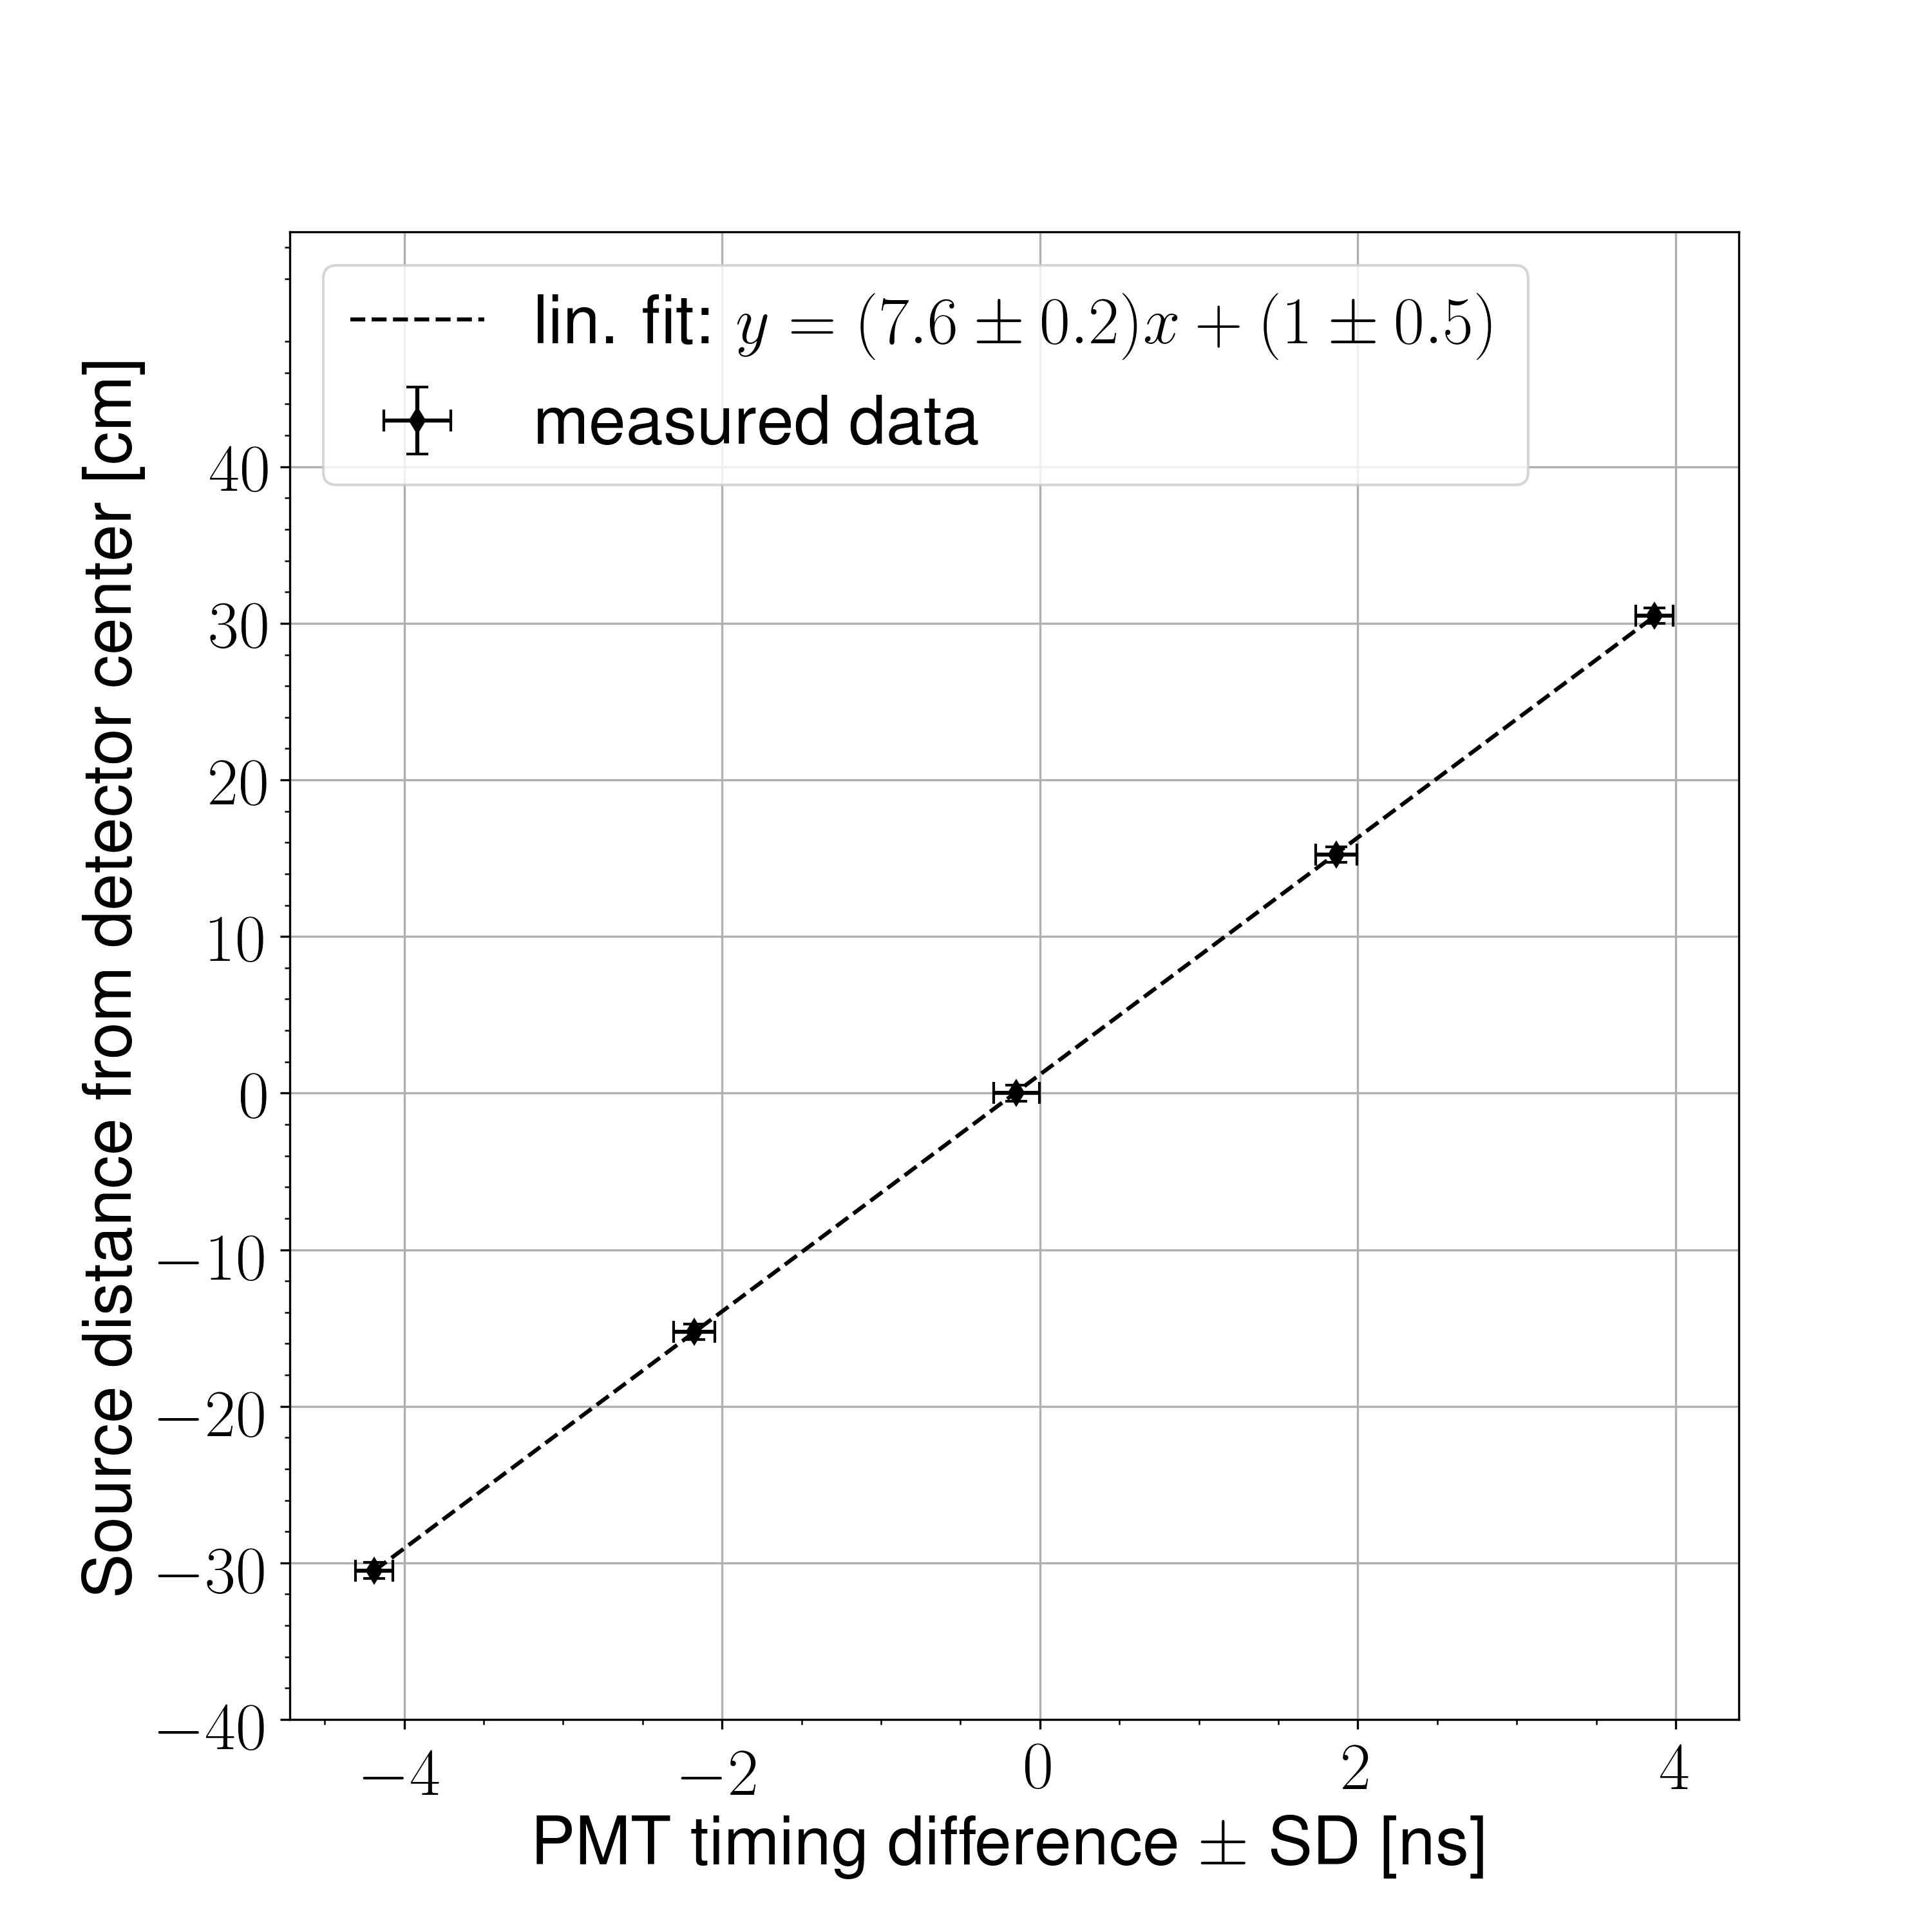
\includegraphics[width = 0.9\textwidth]{Content/Methods/PMTDifference.png}
    \caption{Using a collimated $^{60}Co$ source to produce events at a precise location on the detector, the particle's position along the detector's length is shown to vary linearly with respect to the timing difference between events in the top and bottom PMTs of a detector.}
    \label{fig:PMTDifference}
\end{figure}
\subsubsection{Detector Shielding}
** ToDo: Expand this section and add figures. 

The detector's shielding was designed with the aim of reducing cross-talk, the detection of photons, and noise.
The front face of the detectors, which face towards the target, are subject to the highest flux of gammas due to scatting off the target.
The detection of a gamma renders the detector ``dead'' during the time in which fission neutrons reach the detectors.
Lead readily attenuates gammas, but has the side effect of causing neutrons to scatter and travel an unknown flight path to a detector, which destroys time of flight information.
The extent that neutron flight paths are perturbed due to scattering in the lead shielding was quantified by an MCNP simulation.
Accordingly, 1" of lead was placed along the front face of the detectors.
This effectively diminished gamma detection rates and, according to the simulation, is expected to cause negligible levels of neutron scattering.
Additional lead was used in some special areas that had high gamma flux: at the sides of detectors adjacent to the beam, and along the front faces of the detectors farthest downstream.

Placing lead behind the detectors was avoided in consideration of an MCNP-POLIMI simulation, which indicated that lead placed here facilitates cross-talk. \textit{Cross-talk} is an undesirable phenomenon in which a particle causes a hit in one detector, and then by any means (e.g. scattering), the same particle causes a hit in a different detector.
If both hits occur within the time frame typical for neutrons, then the cross-talk event cannot be distinguished from a true neutron coincidence.
Because cross-talk events are in fact correlated, they cannot be removed in analysis by the subtraction of accidentals.

\subsection{Detector Cross-talk}
**ToDo: Expand this section. Graphs and a more detailed discussion.
The cross-talk plot on the wiki could be insightful.

The geometry of the neutron detector array makes it kinematically impossible for a neutron to scatter from a proton--which is the basis for scintillation--only once within one detector, then travel directly to another detector without undergoing a second scattering event.
Rather, it is kinematically required that a neutron must scatter from at least one intermediate nucleus before traveling into another detector.
This fact can be derived from simple two-body kinematics.
This kinematic requirement alone is not sufficient to neglect the occurrence of cross-talk, because the detectors and the shielding contain significant levels of carbon, lead, and other nuclei, which can function as intermediate scattering points.
To address this, a detailed MCNP-POLIMI simulation was performed that modeled the entire neutron detector array, detector shielding and the supporting structures, and the experimental cell containing it all.
Neutron detection physics was modeled to the point of neutron light output in MeVee, but did not include the propagation of scintillation light or its detection by the PMT tubes.
A distinct feature of MCNP-POLIMI, which is not included in the standard MCNP release, is its ability to model a $^{252}$Cf spontaneous fission source that emits neutrons with the correct correlations.
The detection rate of correlated two-neutron events, relative to the rate of detected cross-talk events, is found by tracking fission neutrons individually through the geometry.
In the simulation, coincident events were detected at a rate that is 36 times greater than for cross-talk events, which is less than a 3\% effect.
Accordingly, no attempt was made to correct for cross-talk in the final result.


\subsection{Targets}
A depleted uranium (DU) target with dimensions of 4x2x0.0.05 $\text{cm}^3$ was used as the primary target for the measurement of two-neutron correlations. DU received the majority of the allotted beam time because it is an even-even nucleus, and as a consequence, has an anisotropic angular distribution of its fission fragments.

One consideration for the target dimensions is the rate of neutron scattering in the target. This has the potential to be a major problem, since a scattering event changes the neutron's direction of the travel and thus creates two-neutron opening angles that are not reflective of what the opening angle was immediately after fission. This effect cannot be eliminated completely, but the target must have small enough dimensions such that the effects of neutron scattering can be neglected. The probability that a two-neutron event is undisturbed by scattering is calculated by squaring the probability that a single neutron is not disturbed. The probability that a single neutron is not disturbed is calculated by an MCNP simulation in which neutrons with an energy spectrum typical of fission neutrons are sample uniformly within a target.

It is desirable to have a target with a symmetry that is consistent with the cylindrical symmetry of the neutron detector array. To accomplish this, a thin rectangular target was rotated slowly about the vertical axis during data acquisition. In doing so, cylindrical symmetry is preserved in the final result, since the final result is an average taken from events which occurred over a long period of time. 

\subsection{Elastic Scattering in Target}
**ToDo: Expand on this section. Discuss MCNP simulation and add a relevant plot. 

MCNP simulations indicated that the probability of a photo-neutron produced in the target escaped without scattering was 97.5\%. Because two neutrons are required for the formation of an opening angle, the rate of data contamination due to scattering is $(1-.975^2)$, or 5\% of two-neutron events.  


\subsection{Measurements with $^{252}$Cf}
**ToDo: reread this and revise.
Maybe place result and comparison of Cf measurements here instead of in results?

Opening angle measurements were also performed on neutrons from the spontaneous fission of $^{252}Cf$.
The configuration for this measurement must be different than that for photofission measurements, as the photon beam can no longer be used as the timing ``start'' trigger.
The trigger for $^{252}Cf$ consisted of two high timing resolution scintillation photon detectors, one fixed below and above the source at a distance of 15 cm.
A 2-fold coincidence between both photon detectors, with a coincidence window of $\Delta t\leq 4$ ns, served as the timing start trigger.
After a new start trigger is implemented, the analysis that follows is equivalent to that of photofission.

As opposed to the measurement of neutrons from photofission, when using neutrons from $^{252}$Cf, there is no concern of accidental neutron pairs.
Given the strength of the source, it is extremely unlikely for two fissions to occur during the neutron time of flight window, thus all detected neutron pairs are expected to be correlated.
Another difference between the two measurements is the clean and sharp peak produced by fission photons from $^{252}$Cf, compared to the relatively smeared peak produced by photons scattering from the target during the photofission measurement.
In both cases, the photon peak is used as a reference point for the time of flight of neutrons, so $^{252}$Cf has less error due to this effect.
The normalization technique used in each case is the same, in which a correlated distribution is divided by an uncorrelated distribution.
Because the opening angle distribution of neutrons from the spontaneous fission of $^{252}$Cf has been measured several several times with good agreement, its measurement in this study gives a good opportunity to verify the validity of the analysis techniques used.

\section{Data Analysis}
\label{Analysis}
The efficiency and acceptance of the neutron detector array varies greatly over the range of opening angles from 0 to 2$\pi$ (see figure~\ref{fig:OpeningAngleAcceptance}a).
This effect is due to the detector array's non-spherical symmetry, and to varying efficiency as a function of particle position.
There was no attempt to measure the array's efficiency as a function of two-neutron opening angle, because it is not necessary and would have been a difficult task.
In this experiment, angular correlation is calculated by normalizing each measurement to an equivalent distribution of uncorrelated neutrons, giving a result that is insensitive to detector efficiencies (see figure~\ref{fig:OpeningAngleAcceptance}b).
The equivalent uncorrelated distribution is formed from a set of manufactured two-neutron events, in which each neutron is taken from a different pulse.
The opening angles between the neutrons are then calculated as normal.
Such pairs will hereafter be referred to as different pulse (DP) pairs.
The neutrons of a DP pair are uncorrelated because events in one pulse do not have casual influence on the events in another pulse.
Detector efficiency and geometry influence same pulse (SP) events and different pulse events equally.
% ToDo: Will be challenging, but further explain why the above statement holds true.
Thus, barring two-neutron correlations and a scaling factor, the DP distribution is identical to the SP distribution.
Each pair of pulses is chosen such that the two pulses occurred within less than a few 100 ms of each other.
This ensures that both pulses are subject to the same experimental conditions, thereby lessening systematic effects from time varying factors such as high-voltage drift and varying beam current.
As many pairs as needed can be readily selected until good counting statistics is achieved, because the only restriction for selecting pulse pairs is that they occurred around roughly the same time.
% ToDo: Compare our result for CF252 to another result. Overlay with this figure.
\begin{figure}
    \centering
    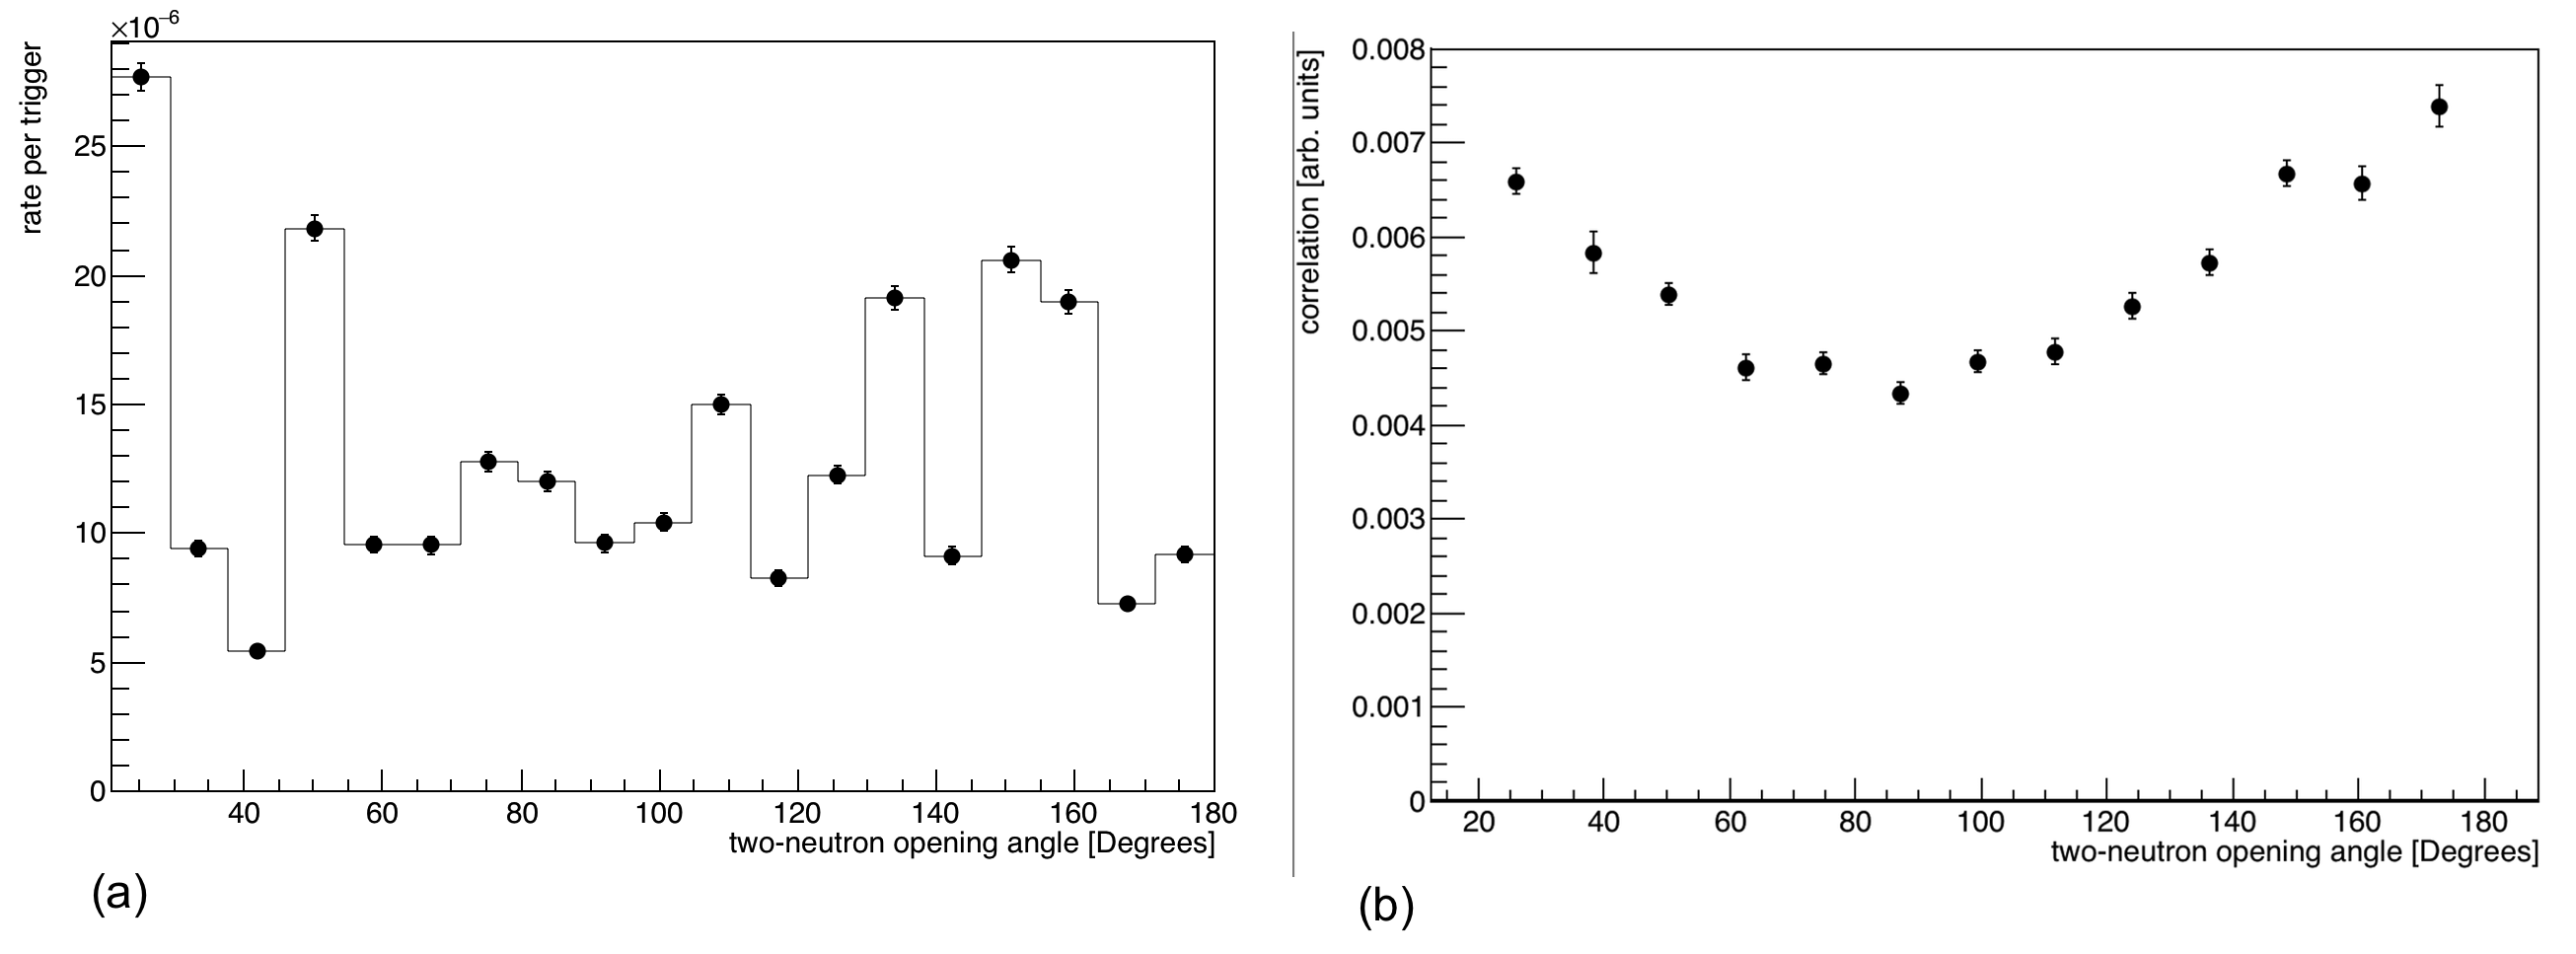
\includegraphics[width  = \textwidth ]{Content/Methods/Normalization.png}
    \caption{(a) Unnormalized two-neutron opening angle distribution from the spontaneous fission of $^{252}$Cf. The structure is reflective of geometric acceptance and efficiencies. (b) Same distribution after division by uncorrelated two-neutron events, which are taken from different pulses.}
    \label{fig:OpeningAngleAcceptance}
    \label{fig:OpeningAngleAcceptance}
\end{figure}
\subsection{Subtraction of Accidentals}
\label{Subtraction of Accidentals}
An accidental neutron coincidence is defined as a coincidence between two uncorrelated events in a single pulse.
For example, a coincidence between a neutron from a (gamma,1n) reaction and a neutron from photofission.
Another example is a coincidence between two events that are part of the noise background.
In both of these examples, the two events are considered accidentals because they have no causal influence on each another.
A true neutron coincidence, or true for short, is defined here as any pair correlated neutrons from the same pulse.

Accidentals are removed from the data by subtracting 1/2 times the equivalent distribution formed by the DP data.
The factor of 1/2 arises from the Poissonian statistics that inherently govern all accidentals, whether the accidental events are composed of two neutrons, two photons, two noise events, or any combination thereof.
% ToDo: Explain why the use of Poissonian statistics is valid.
An accidental is comprised of the occurrence of two independent events.
Therefore, as per Poissonian statistics, the probability of measuring an accidental in a single pulse is given by:
\begin{displaymath}
SP_{\text{a}} = \frac{e^{-\lambda}\lambda^2}{2} \approx \frac{1}{2}\lambda^{2}
\end{displaymath}
where $SP_{a}$ is the accidental rate of single pulses, $\lambda$ is the mean accidental rate of single pulses–an unknown value.
In this study, the coincidence rates were around $5\times10^{-5}$ events per pulse, so the approximation used above is correct to within 0.001\% as the worst case scenario.
Since the DP data is formed by observations of events from two different pulses, the DP accidental rate is equal to the Poissonian probability of one event, squared.
\begin{displaymath}
DP_{\text{a}} = (e^{-\lambda}\lambda)^{2}\approx \lambda^{2} 
\end{displaymath}
where $DP_{\text{a}}$ is the accidental rate of DP events.
Therefore, if coincidence rates, then the rate of measured accidentals in single pulses is 1/2 times the rate of accidentals in the different pulses.
In this study the subtraction had about a ten percent effect.






\chapter{Discussion of Experimental Errors}
\label{Errors}
\section{Resolution of measurement}
The position of a detected particle is known to within a specified distance, which translates into a resolution in the measurement of the opening angle between a pair of particles.
A particle's reconstructed position along a detector's length has an error of $\pm$13 cm.
Due to the detector's 15 cm width, there is also a positional uncertainty of $\pm 7.5$ cm in the direction perpendicular to the detector's length.
The amount of uncertainty in a single two-neutron opening angle measurement is determined from of the uncertainties in the positions of each detected neutron.
These positional uncertainties are propagated through the formula for the calculation of opening angle, which is
\begin{displaymath}
    \theta_{nn} = \text{arccos}\left(\frac{\vec{v_{1}}^{\,}\cdot\vec{v_{2}}^{\,}}{|\vec{v_{1}}^{\,}||\vec{v_{2}}^{\,}|}\right)
\end{displaymath}
where $\vec{v_{1}}^{\,} = (x_1,y_1,z_1)$ and $\vec{v_{2}}^{\,} = (x_2,y_2,z_2)$ are the detected positions of the two neutrons.
The propagation of error through this formula is achieved by evaluating the following expression
\begin{eqnarray}
\label{eq:propagation}
 \Delta \theta_{nn} & = & \left( \left(\Delta x_1 \frac{\partial \theta}{\partial x_1}\right)^{2} + \left(\Delta y_1 \frac{\partial \theta}{\partial y_1}\right)^{2} + \left(\Delta z_1 \frac{\partial \theta}{\partial z_1}\right)^{2} + \right. \\
 & & \left. + \left(\Delta x_2 \frac{\partial \theta}{\partial x_2}\right)^{2} + \left(\Delta y_2\frac{\partial \theta}{\partial y_2}\right)^{2} + \left(\Delta z_2 \frac{\partial \theta}{\partial z_2}\right)^{2} \right) ^{\frac{1}{2}} \, ,  \nonumber
\end{eqnarray}
where the $\Delta$'s represent the uncertainty in the variable that directly follows each $\Delta$.
The values and uncertainties of all events in a given angle bin are fed through Eq.\ref{eq:propagation}, and then averaged together.
The result, seen in Fig.~\ref{fig:OpeningAngleRes}, can be interpreted as the opening angle resolution as a function of $\theta_{nn}$.
\begin{figure}[h]
    \centering
    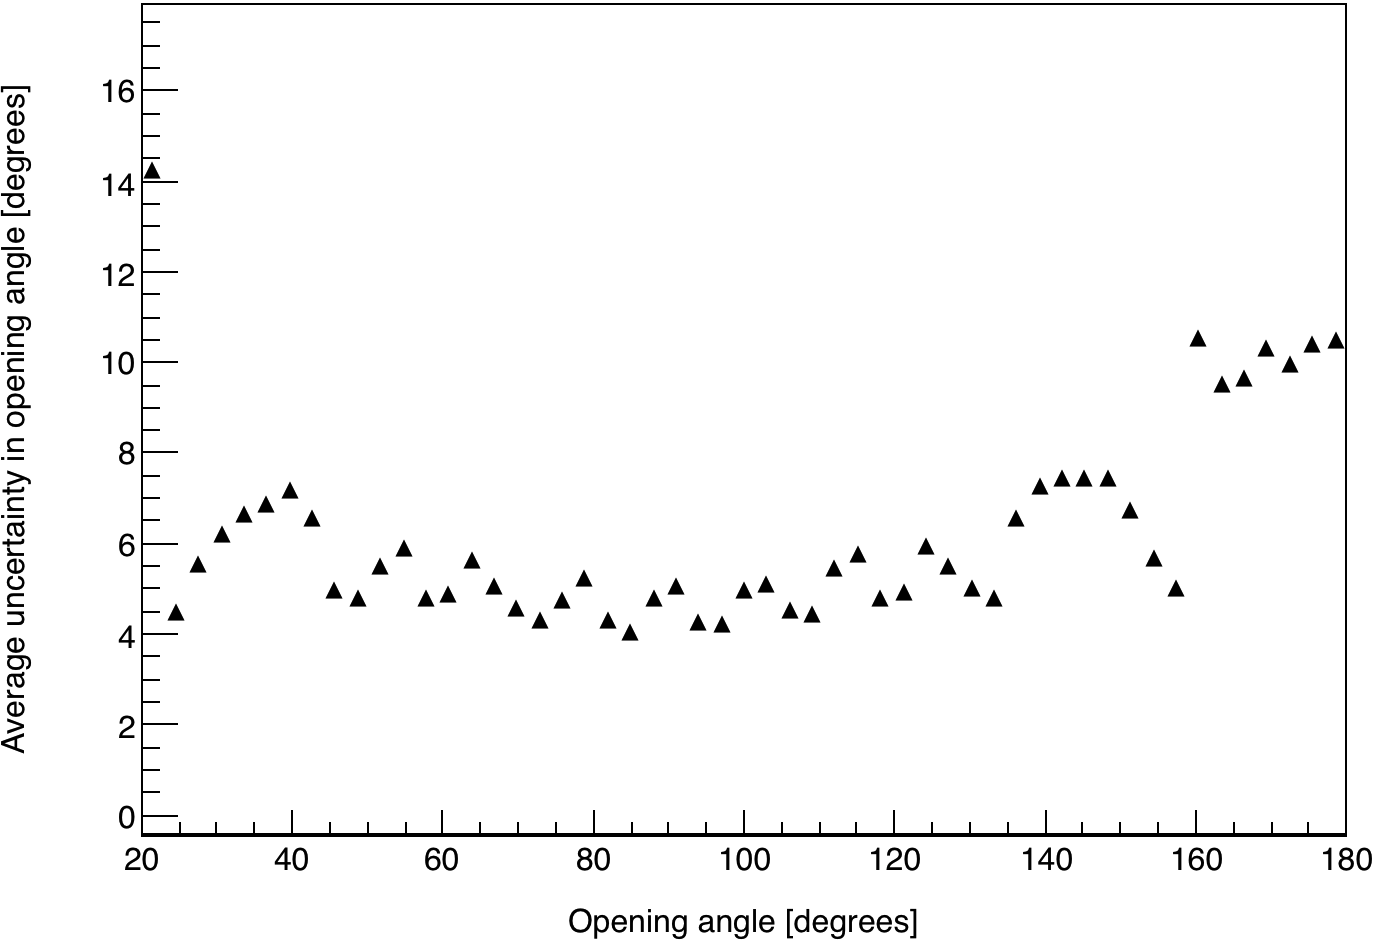
\includegraphics[width = 0.85\textwidth]{Content/Errors/OpeningAngleUncertainty.png}
    \caption{Uncertainties in opening angle determined from the propagation of position uncertainties through the opening angle calculation.
     The uncertainty of a given opening angle measurement depends on which detectors are involved and the position of the particles on the detectors.
     For this reason, the uncertainty of measurements falling within each angle bin is a distribution, so the average uncertainties are plotted here.
    The y-axis can be viewed as a measure of angular resolution in the sense that it represents the smallest angular difference that can be considered statistically significant.
    }
    \label{fig:OpeningAngleRes}
\end{figure}

\section{Counting error}
The uncertainty in the number of observed events is always assumed to be equal to $\sqrt{N}$, as per Poissonian  statistics, where N is the number of observed events.
This value is then propagated through all the analysis procedure using the standard methods for the propagation of error.
The vertical error bars seen in all results are due solely to such counting error.

\FloatBarrier
\section{Detector Cross-talk}
\label{crosstalk}
\textit{Cross-talk} occurs when, after a particle is detected once, the same particle, by any means, causes a detection to be registered in a different detector.
For example, upon detection, a particle may undergo elastic scattering and then travel into a another detector where it is detected again, or it may produce secondary particles that are detected.
The two coincident detections of a cross-talk event are causally correlated, and thus they have the potential to contaminate the signal from correlated fission neutrons.
If both detections occur during the ToF range typical for fission neutrons, then the cross-talk event cannot be distinguished from the detection of two correlated neutrons.

Recent works that measured the two-neutron angular correlations in the spontaneous fission of $^{252}$Cf and $^{240}$Pu~\cite{Pozzi2016,Verbeke2018} addressed this effect by using an MCNP-PoLiMi simulation to estimate and then subtract cross-talk from their measurements.
In this work, the issue of cross-talk is approached differently by employing the use of detector shielding aimed at reducing cross-talk to a negligible rate.
By using shielding to reduce cross-talk, this measurement is less dependent on the details of the models used by MCNP-PoLiMi to simulate neutron transport and detection.
MCNP-PoLoMi simulations are used in this work only to verify that the effect of cross-talk is negligible.
The scintillators used here are much larger than those used in similar works, such as in refs~\cite{Pozzi2016,Verbeke2018}, allowing for them to be placed much farther from the fission source without causing extremely low coincidence rates. 
An increase in the distance between the detectors and the fission source makes this measurement less sensitive to angular uncertainty, which is influenced by the uncertainty in the position of a detected particle due to, for example, the scattering of neutrons from detector shielding.
Because of this, larger amounts of shielding can be used without concern of introducing large errors.

The geometry of the neutron detection system makes it kinematically impossible for a neutron to scatter from a proton in one detector--which is the basis for scintillation--and then travel directly into another detector with enough kinetic energy to be detected a second time.
For this reason, upon being detected, a neutron must scatter from one or more intermediate nuclei, such as Pb or C, in order for it to reach a different detector with enough energy to be detected a second time.
This fact follows from the conservation of energy and momentum.
Figure~\ref{fig:CrossTalkExample} illustrates a cross-talk event due to a neutron scattering in a detector's shielding.
In order to be more convinced that such events occur at negligible rates, a detailed MCNP-PoliMi~\cite{MCNP_POLIMI} simulation was performed to model cross-talk.
\begin{figure}
    \centering
    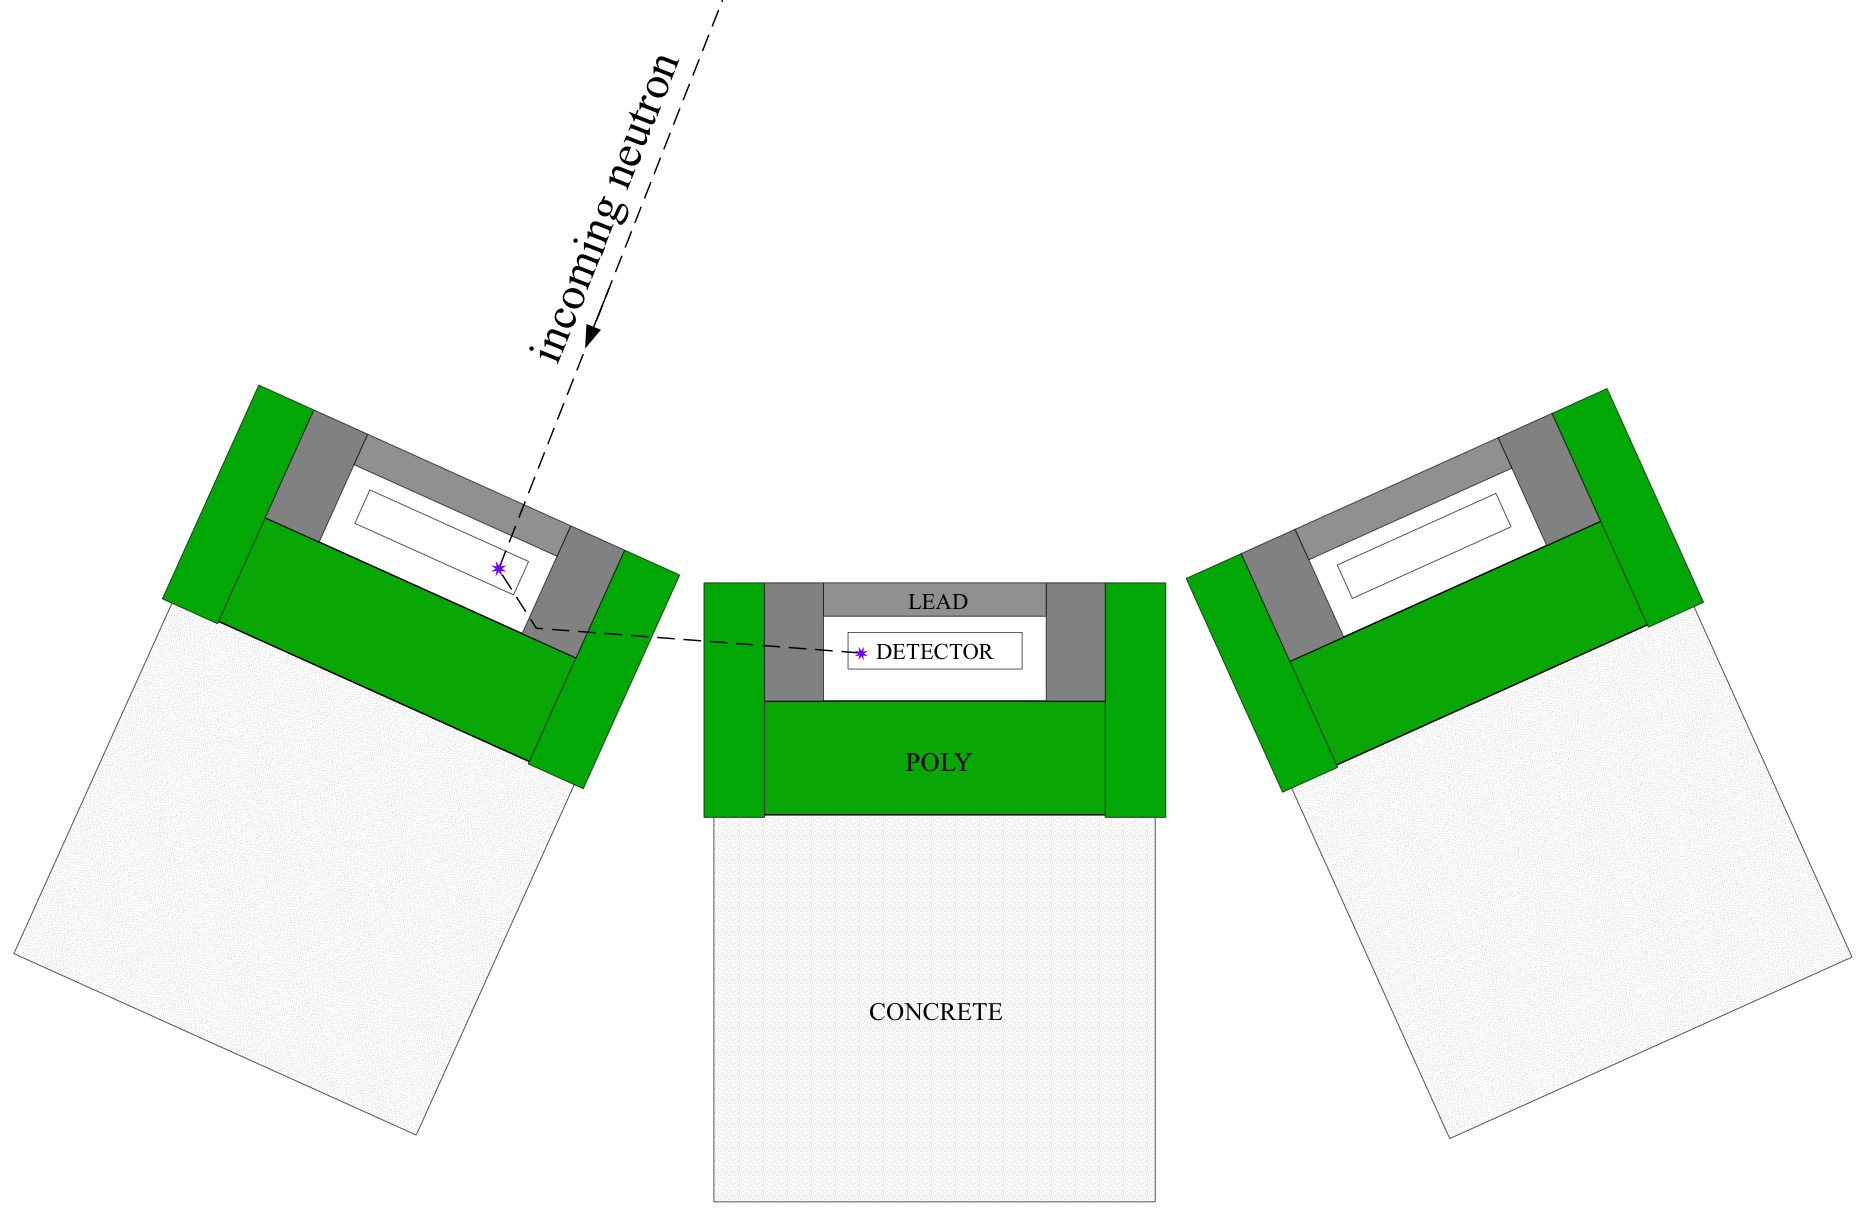
\includegraphics[width = 0.95\textwidth]{Content/Errors/CrossTalkExample.png}
    \caption{A hypothetical example of a neutron cross-talk event.
An incoming neutron is detected and then scatters from some lead shielding nearby, which changes its direction of travel such that it enters a second detector where it is detected a second time.
The scattering of a neutron from an intermediate nucleus, in this example a lead nucleus, is kinematically required in order for cross-talk to occur in this experiment.}
    \label{fig:CrossTalkExample}
\end{figure}

\section{Simulation of Detector Cross-talk}
A simulation was performed to ensure that the detector shielding effectively reduced cross-talk to negligible levels.
The simulation included all scintillators and their shielding, supporting structures, and the concrete walls surrounding the experimental cell.
MCNP-PoliMi's built-in $^{252}$Cf spontaneous fission source was used, which emits neutrons with the correct correlations and multiplicities.
Detector response was modeled using a program included with the MCNP-PoliMi distribution called MPPost~\cite{MPPost}.
The model is based on the electron equivalent light output (MeVee) produced by particles as they undergo collisions with carbon and hydrogen within organic plastic scintillators.
A minimum deposited energy of 0.4 MeV ( 0.05 MeVee for neutrons) was assumed for detectable particles, which was chosen because the neutron detection system showed a sharp decline in detection rates for neutrons below 0.4 MeV.
For neutron collisions with hydrogen, the light output in MeVee, $L$, is calculated by the following empirically derived formula
\begin{displaymath}
L = 0.0364 E_n^2 +  0.125 E_n
\end{displaymath}
where $E_n$ is equal to the loss in the kinetic energy of the neutron due to the collision.
Neutron interactions with carbon are assumed to generate a small light output of
\begin{displaymath}
L = 0.02 E_n
\end{displaymath}
As seen in Fig.~\ref{fig:Cf252MCNPVsEXP}, this model produces a ToF spectrum that is in good agreement with the measurement.
\begin{figure}
    \centering
    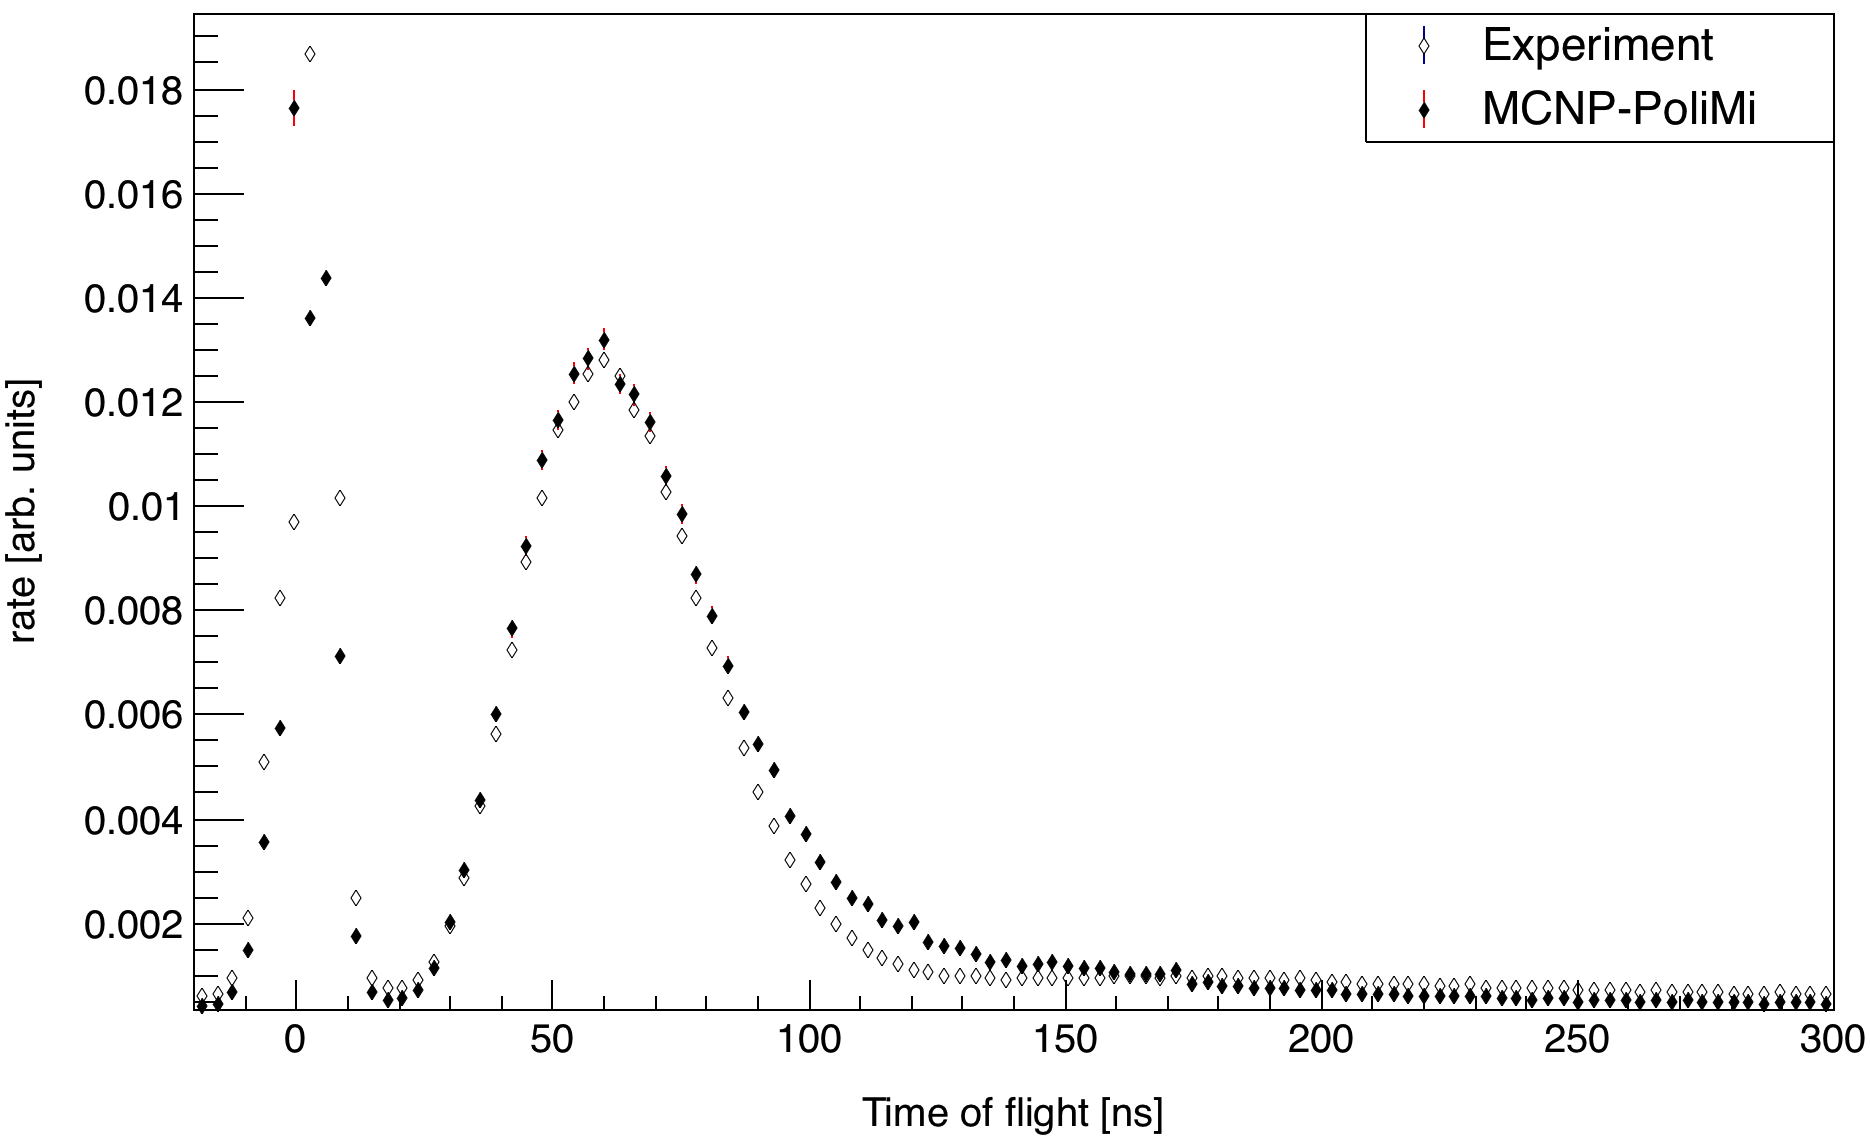
\includegraphics[width = 0.9\textwidth]{Content/Errors/Cf252MCNPVsEXP.png}
    \caption{Measured \emph{versus} simulated ToF spectrum of a $^{252}$Cf spontaneous fission source. 
    The simulation also used a detector response model based on ref~\cite{MPPost}}
    \label{fig:Cf252MCNPVsEXP}
\end{figure}

The simulation was initially performed with 5 cm of lead shielding placed behind the scintillators, and the number of cross-talk events accounted for 11\% of the total coincident neutron events.
The amount of cross-talk fell to 3\% if polyethylene was used instead of lead, which motivated the placement of 10~cm of polyethylene behind the detectors during construction.
Figure~\ref{fig:CrosstalkVScoincidence} shows the distribution of cross-talk events and true two-neutron coincidences as a function of reconstructed opening angle.
It is worth noting that, according to the simulation, the effect of cross-talk is not only small, but is also distributed over a wide range of angles rather than being concentrated around $\theta_{nn}=0$.
Angles greater than 125 degrees are not shown in Fig.~\ref{fig:CrosstalkVScoincidence}, because these cross-talk events can be readily identified in analysis by the large amount of time required for a neutron to travel the required distances.
\begin{figure}
    \centering
    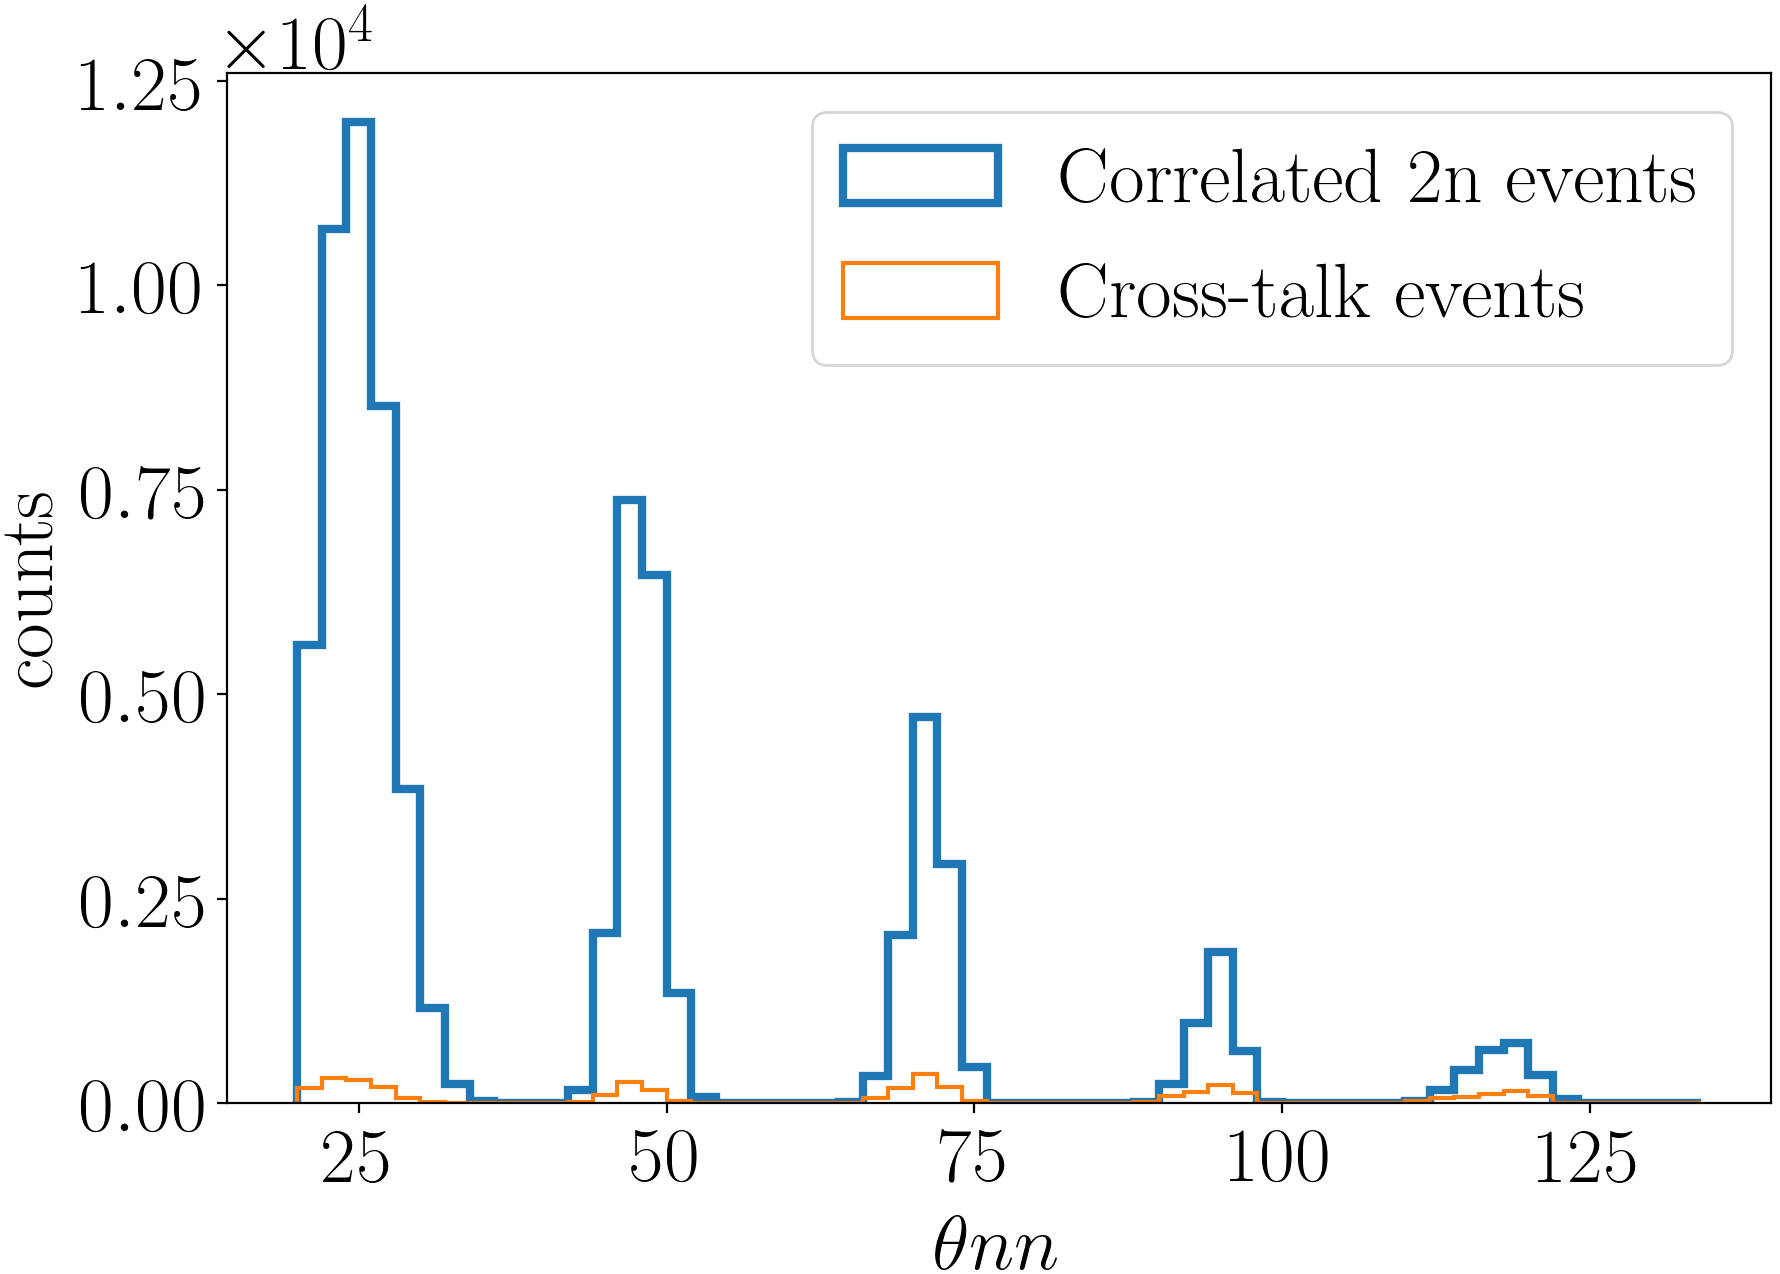
\includegraphics[width = 0.95\textwidth]{Content/Errors/CrosstalkVScoincidence.png}
    \caption{
    MCNP-PoLiMi simulation of the number of cross-talk events \emph{versus} correlated two-neutron events as a function of reconstructed opening angle.
    Cross-talk accounted for 3\% of total events.
    In this work, cross-talk does not occur primarily at small angles, but is instead spread out over a wide range of angles.
    }
    \label{fig:CrosstalkVScoincidence}
\end{figure}

\section{Neutron Scattering within Target}
\label{subsection:Elastic_scattering}
A potential source of error in opening angle measurements is the scattering of neutrons within the fission target.
This is a cause for concern, because a neutron that scatters from a heavy nucleons is very likely to be deflected at a large angle, creating two-neutron opening angles that are not reflective of the true opening angle immediately after fission.
Furthermore, because the target used in this work has the shape of a thin strip, it is more likely that neutrons that are initially traveling towards a given detector are deflected away by scattering if said detector is aligned along the wide (2~cm) axis of the strip, as opposed to the thin (0.05~cm) axis.
This bias is removed by slowly rotating the target about the vertical axis during data acquisition.
Because the subject of this measurement is fundamentally a statistical process, useful interpretations of the data are average rates taken over many events.
Thus, by rotating the target, cylindrical symmetry is preserved in the average, producing a result equivalent to that if a cylindrical target were used.

A thin strip is the ideal target shape regarding the rate of neutron elastic scattering per unit volume.
See Fig~\ref{fig:ElasticScatteringPlot} for the result of an MCNP simulation of the elastic scattering rates for both thin strip and cylindrical shaped targets.
The target in this experiment was a thin strip with a width 40 times greater than its thickness, for which the simulation indicated the rate of elastic scattering is roughly a factor of two less than for a cylindrical target of the same volume.

The target's dimensions are small enough that the rate of photon absorption, and thus photo-neutron production, is virtually uniform throughout the entire target volume.
MCNP was used to simulate the production of pairs of fission neutrons uniformly throughout the target volume with energies typical of fission neutrons.
The probability that at least one neutron out of a pair of two scatters before exiting the target was calculated from the simulation.
For the target used in this work, the simulation indicated that 6\% of two-neutron opening angles were altered due to scattering.
\begin{figure}
    \centering
    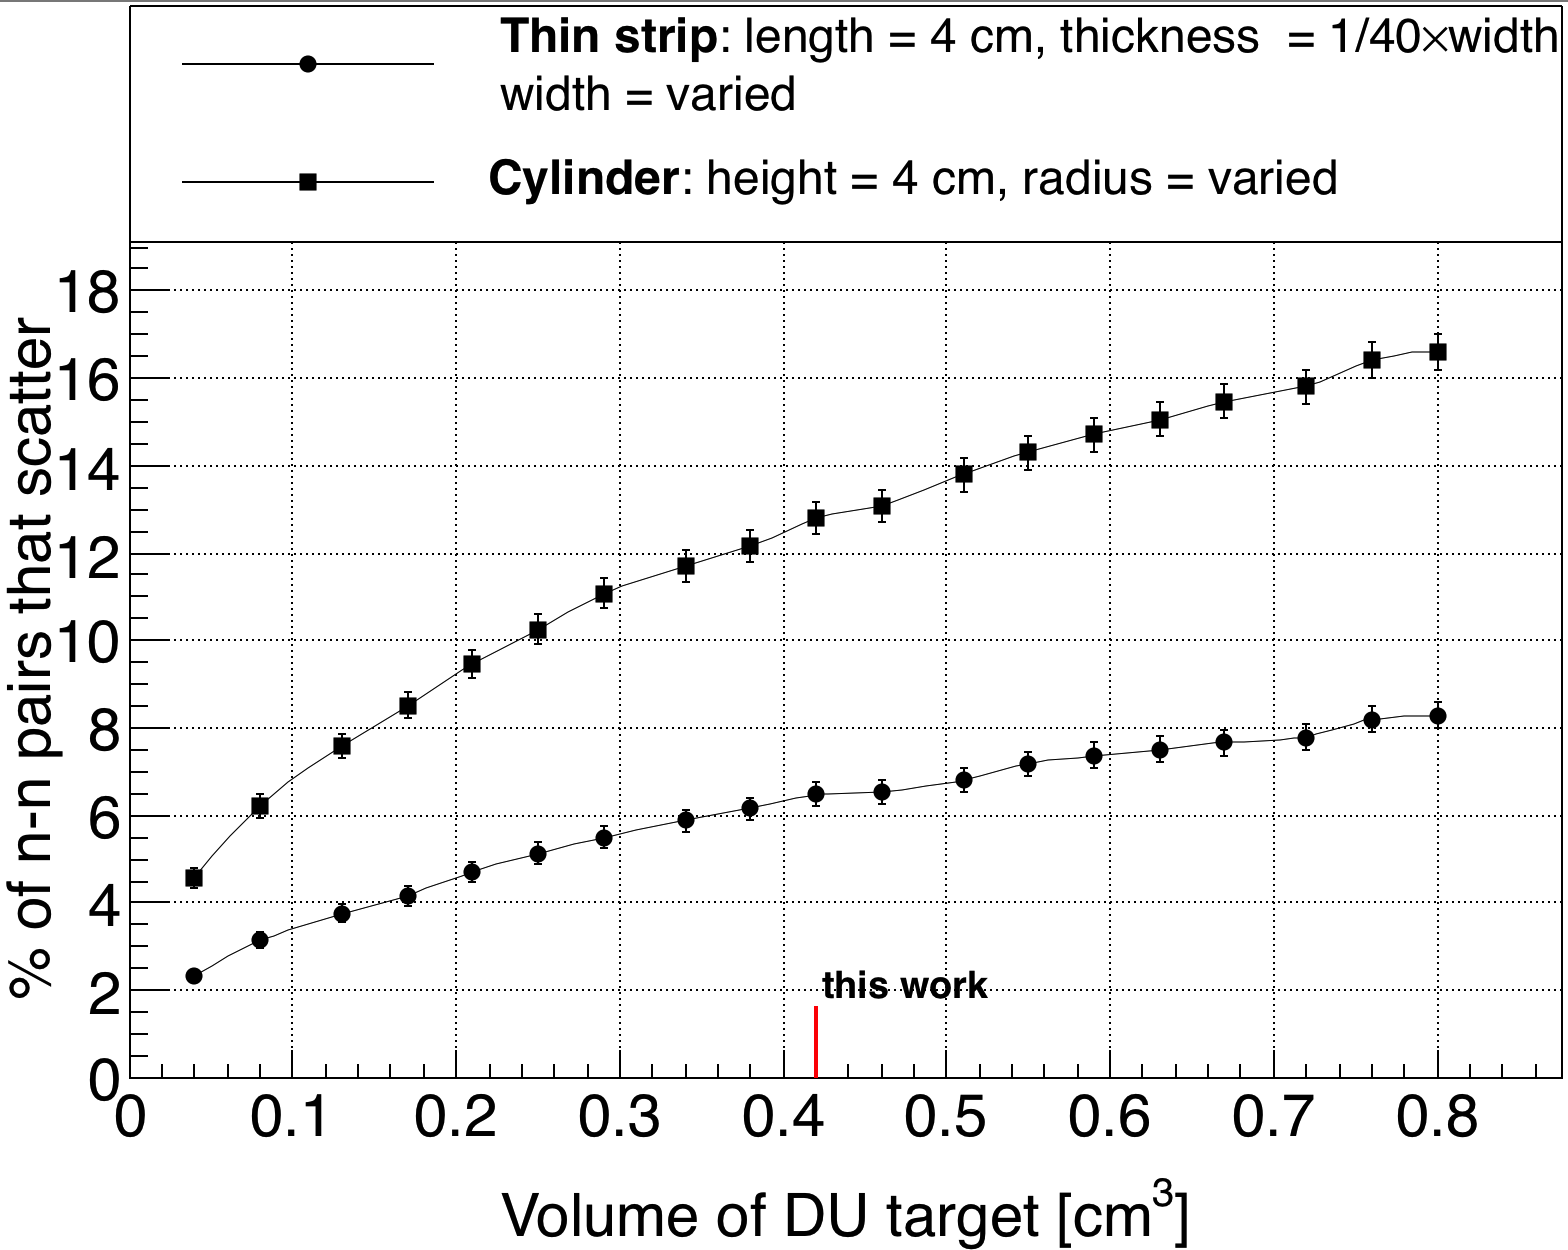
\includegraphics[width = 0.95\textwidth]{Content/Errors/ElasticScatteringPlot.png}
    \caption{
     Result of an MCNP simulation in which neutron-neutron pairs, with energies sampled from a typical watt fission spectrum, were generated uniformly throughout the volume of DU targets.
        The y-axis is the rate of opening angle contamination due to the scattering of, within the DU target in which they were produced, either one or both of a pair of neutrons.
    The lack of symmetry of a thin strip target can be removed by slowly rotating the target around the vertical axis during data acquisition, making it the optimal target geometry for the minimization of the rate of neutron scattering.
    The target used in this work had a length of 4~cm, a width of 2~cm, and a thickness of 0.05~cm.
    }
    \label{fig:ElasticScatteringPlot}
\end{figure}

\chapter{Results}



\chapter{Concluding Remarks}
Two-neutron angular correlations in the photofission of $^{238}$U were measured using 10.5 MeV end-point bremsstrahlung photons produced via a low duty factor, pulsed linear electron accelerator.
The measured angular correlations reflect the underlying back-to-back nature of the fission fragments.
The method of analysis uses a single set of experimental data to produce a opening angle distribution of correlated and uncorrelated neutron pairs.
A ratio is taken between these two sets to provide a self-contained result of angular correlations that is independent of neutron detector efficiencies.
Two-neutron angular correlation measurements were also made using neutrons from the SF of $^{252}$Cf and are in good agreement with previous measurements.

Measured two-neutron opening angular correlations were in fair agreement with simulations that used FREYA version 2.0.3, which uses a neutron-induced model to approximate photofission.
These data will be useful for fine-tuning the photofission models that will be incorporated into future versions of FREYA.

An anomaly was observed in the rate of neutron emission at opening angles near 180$^{\circ}$, in which diminished rates resulted in a local maximum at about 160$^{\circ}$ instead of the expected 180$^{\circ}$ as seen in all past measurements of neutron-induced and spontaneous fission.
We offer two possible explanations for this effect:
\begin{enumerate*}[label=(\roman*), itemjoin={{, }}, itemjoin*={{, or }}]
  \item There is a decrease in neutron emission along the fission axis
  \item the neutrons may indeed be emitted isotropically in the rest frame of the fission fragment, but one fragment essentially shadows the neutrons emitted from the other fragment, either through absorption or scattering.
  \end{enumerate*}
A definitive interpretation of this decreased two-neutron correlation for large opening angles in photo-fission requires further study.

\appendix

\chapter{Appendix}
\thispagestyle{fancy}
\section{Rates}
\label{sec:rates}
Table~\ref{table:rates} shows the rates, per pulse, of the detection of photons and neutrons for each detector.
The overall rate of neutron singles and doubles was 4.89$\times 10^{-3}$ and 3.57$\times 10^{-5}$ per pulse, respectively.
\begin{center}
 \begin{table}
 \centering
\begin{tabular}{c  S[table-format=1.4e-2] S[table-format=1.4e-2]}%S[table-format=1.4]} %{||c |c |c |c| c||}  ccS[table-format=1.4e-2]
 \toprule
\textbf{Detector} & \textbf{neutron rate} & \textbf{photon rate} \\ [0.5ex] 
\midrule
30 bottom & 4.43E-04 & 1.93E-01 \\ \midrule
30 top & 2.11E-04 & 1.68E-01 \\ \midrule
54 & 5.03E-04 & 3.77E-01 \\ \midrule
78 & 4.27E-04 & 9.67E-02 \\ \midrule
102 & 3.61E-04 & 4.73E-02 \\ \midrule
126 & 7.13E-04 & 5.14E-02 \\ \midrule
150 & 5.76E-04 & 3.79E-02 \\ \midrule
210 & 7.16E-04 & 4.99E-02 \\ \midrule
234 & 4.49E-04 & 4.49E-02 \\ \midrule
258 & 5.27E-04 & 5.90E-02 \\ \midrule
282 & 4.42E-04 & 1.04E-01 \\ \midrule
306 & 3.40E-04 & 3.17E-01 \\ \midrule
330 bottom & 3.46E-04 & 2.35E-01 \\ \midrule
330 top & 3.24E-04 & 2.50E-01 \\
\bottomrule
\end{tabular}
\caption{
Per pulse rate of neutrons and photons on each detector.
Only one particle can be detected by a given detector per pulse, so the rate of photon detection affects the measured neutron rate.
}
  \label{table:rates}
\end{table}
\end{center}


\backmatter

\bibliographystyle{plain}
\bibliography{./refs.bib}


\end{document}